\title{ソーシャルブックマーキングサービスのデータ分析によるウェブマーケティング}
\author{プロジェクトマネジメントコース\\
ソフトウェア開発管理グループ\\
矢吹研究室\\
1342029\\
遠藤一輝}
\date{}
\begin{document}
\maketitle

%本テンプレートの余白は,卒論マニュアルで指示されたものとは違っているが,1ページあたりの文字数は40文字x40行と,卒論マニュアル通りになっている。文字間隔や行間隔を調整して,余白をマニュアル通りにすることもできるが,それでは文章が読みにくくなるため,このような対応をしている。

%\noindent
□□□□□□□□□■□□□□□□□□□■□□□□□□□□□■□□□□□□□□□■
□□□□□□□□□■□□□□□□□□□■□□□□□□□□□■□□□□□□□□□■
□□□□□□□□□■□□□□□□□□□■□□□□□□□□□■□□□□□□□□□■
□□□□□□□□□■□□□□□□□□□■□□□□□□□□□■□□□□□□□□□■
□□□□□□□□□■□□□□□□□□□■□□□□□□□□□■□□□□□□□□□■
□□□□□□□□□■□□□□□□□□□■□□□□□□□□□■□□□□□□□□□■
□□□□□□□□□■□□□□□□□□□■□□□□□□□□□■□□□□□□□□□■
□□□□□□□□□■□□□□□□□□□■□□□□□□□□□■□□□□□□□□□■
□□□□□□□□□■□□□□□□□□□■□□□□□□□□□■□□□□□□□□□■
□□□□□□□□□■□□□□□□□□□■□□□□□□□□□■□□□□□□□□□■
□□□□□□□□□■□□□□□□□□□■□□□□□□□□□■□□□□□□□□□■
□□□□□□□□□■□□□□□□□□□■□□□□□□□□□■□□□□□□□□□■
□□□□□□□□□■□□□□□□□□□■□□□□□□□□□■□□□□□□□□□■
□□□□□□□□□■□□□□□□□□□■□□□□□□□□□■□□□□□□□□□■
□□□□□□□□□■□□□□□□□□□■□□□□□□□□□■□□□□□□□□□■
□□□□□□□□□■□□□□□□□□□■□□□□□□□□□■□□□□□□□□□■
□□□□□□□□□■□□□□□□□□□■□□□□□□□□□■□□□□□□□□□■
□□□□□□□□□■□□□□□□□□□■□□□□□□□□□■□□□□□□□□□■
□□□□□□□□□■□□□□□□□□□■□□□□□□□□□■□□□□□□□□□■
□□□□□□□□□■□□□□□□□□□■□□□□□□□□□■□□□□□□□□□■
□□□□□□□□□■□□□□□□□□□■□□□□□□□□□■□□□□□□□□□■
□□□□□□□□□■□□□□□□□□□■□□□□□□□□□■□□□□□□□□□■
□□□□□□□□□■□□□□□□□□□■□□□□□□□□□■□□□□□□□□□■
□□□□□□□□□■□□□□□□□□□■□□□□□□□□□■□□□□□□□□□■
□□□□□□□□□■□□□□□□□□□■□□□□□□□□□■□□□□□□□□□■
□□□□□□□□□■□□□□□□□□□■□□□□□□□□□■□□□□□□□□□■
□□□□□□□□□■□□□□□□□□□■□□□□□□□□□■□□□□□□□□□■
□□□□□□□□□■□□□□□□□□□■□□□□□□□□□■□□□□□□□□□■
□□□□□□□□□■□□□□□□□□□■□□□□□□□□□■□□□□□□□□□■
□□□□□□□□□■□□□□□□□□□■□□□□□□□□□■□□□□□□□□□■
□□□□□□□□□■□□□□□□□□□■□□□□□□□□□■□□□□□□□□□■
□□□□□□□□□■□□□□□□□□□■□□□□□□□□□■□□□□□□□□□■
□□□□□□□□□■□□□□□□□□□■□□□□□□□□□■□□□□□□□□□■
□□□□□□□□□■□□□□□□□□□■□□□□□□□□□■□□□□□□□□□■
□□□□□□□□□■□□□□□□□□□■□□□□□□□□□■□□□□□□□□□■
□□□□□□□□□■□□□□□□□□□■□□□□□□□□□■□□□□□□□□□■
□□□□□□□□□■□□□□□□□□□■□□□□□□□□□■□□□□□□□□□■
□□□□□□□□□■□□□□□□□□□■□□□□□□□□□■□□□□□□□□□■
□□□□□□□□□■□□□□□□□□□■□□□□□□□□□■□□□□□□□□□■
■■■■■■■■■■■■■■■■■■■■■■■■■■■■■■■■■■■■■■■■
□□□□□□□□□■□□□□□□□□□■□□□□□□□□□■□□□□□□□□□■%文字数チェック用



\chapter*{謝辞}\addcontentsline{toc}{chapter}{謝辞}

本研究の作成において,矢吹研究室矢吹太朗准教授には数多くのご指導,ご鞭撻を賜り深謝致します.また,並びに数多くの助言やご指摘をくださいました矢吹研究室の同期,後輩の皆様に感謝致します.

\tableofcontents%目次

\chapter{序論}
本研究は,ウェブマーケティングに関するデータの分析を行い,ウェブマーケティングの効率的な手法についての考察と提案を行う.\par
インターネットの発展に伴う情報の入手手段の増加と媒体の多様化により,私たちの周りには多くの情報があふれるようになった.
それに伴いマーケティングの手法も新たな体系としてインターネットを利用したウェブマーケティングがうまれた.
様々な媒体から手軽に見られるインターネットは新しいマーケティングの場として適したものであり,多くのマーケティングがウェブ上で行われている.\par
インターネットでは手軽に情報の入手及び発信が行えるが,インターネット上にある情報は膨大なため必要とする情報の取捨選択が求められる.そのため自身の発信する情報を多くの人に閲覧してもらうためには,発信する情報を効果的に伝えることが重要となる.\par
そこでウェブマーケティングを効果的に行うための指標を作成することを目的とし,ウェブマーケティングの分析を行う.

\chapter{背景}
インターネットで情報を得ようとするとき,インターネット上には個人では扱いきれないほどの多くの情報があふれており,必要な情報のみを選択しなければ調査に多くの時間がかかってしまう.\par
そのため私たちは情報を得るとき,情報の様々な要素からその情報が自身に必要なものかを判断し,取捨選択をすることで本当にその情報が自身が必要としているものか見極めている.\par
情報の様々な要素とはタイトルや掲載日時,タグなどの情報発見に必要な情報から詳しい内容やコメント,画像などのそれが自身にとって必要か判断するための情報など多岐にわたる種類のものである.\par
本研究では数多くある要素のうち,時間の推移と閲覧した人数の関係に対して研究を行い,その結果をもとに効果的なウェブマーケティングの手法を考察することで,ウェブマーケティングの一つの指標とすることを目標とする.

\chapter{ソーシャルブックマーキングサービスについて}
本章ではソーシャルブックマーキングサービスについて解説する.

\section{本研究におけるソーシャルブックマーキングサービスの使用の理由について}
本研究においてはウェブマーケティングの一例としてソーシャルブックマーキングサービスを用いる.\par
その理由を以下に挙げる.

\begin{enumerate}
\item 様々な利用者が様々な分野の記事をブックマークに登録するため,幅広い分野のデータが得られる.
\item 不特定多数の人物のブックマークを参考にするため,思惟が関わりにくく偏りが起こりにくい.
\item ウェブマーケティングは幅広い範囲の分野に対応するため,比較のための共通の数値が必要となる.ソーシャルブックマーキングサービスでは,共通の数値であるブックマーク数というデータが得られるため,比較が容易となる.
\end{enumerate}

\newpage

\section{ソーシャルブックマーキングサービスとは}
ソーシャルブックマーキングサービスとは,ユーザーのブックマークをローカルではなくインターネット上に保存するサービスである.\par
インターネット上にブックマークを保存するため,端末が異なってもブックマークを共有できる.\par

\begin{figure}[htb]
\centering
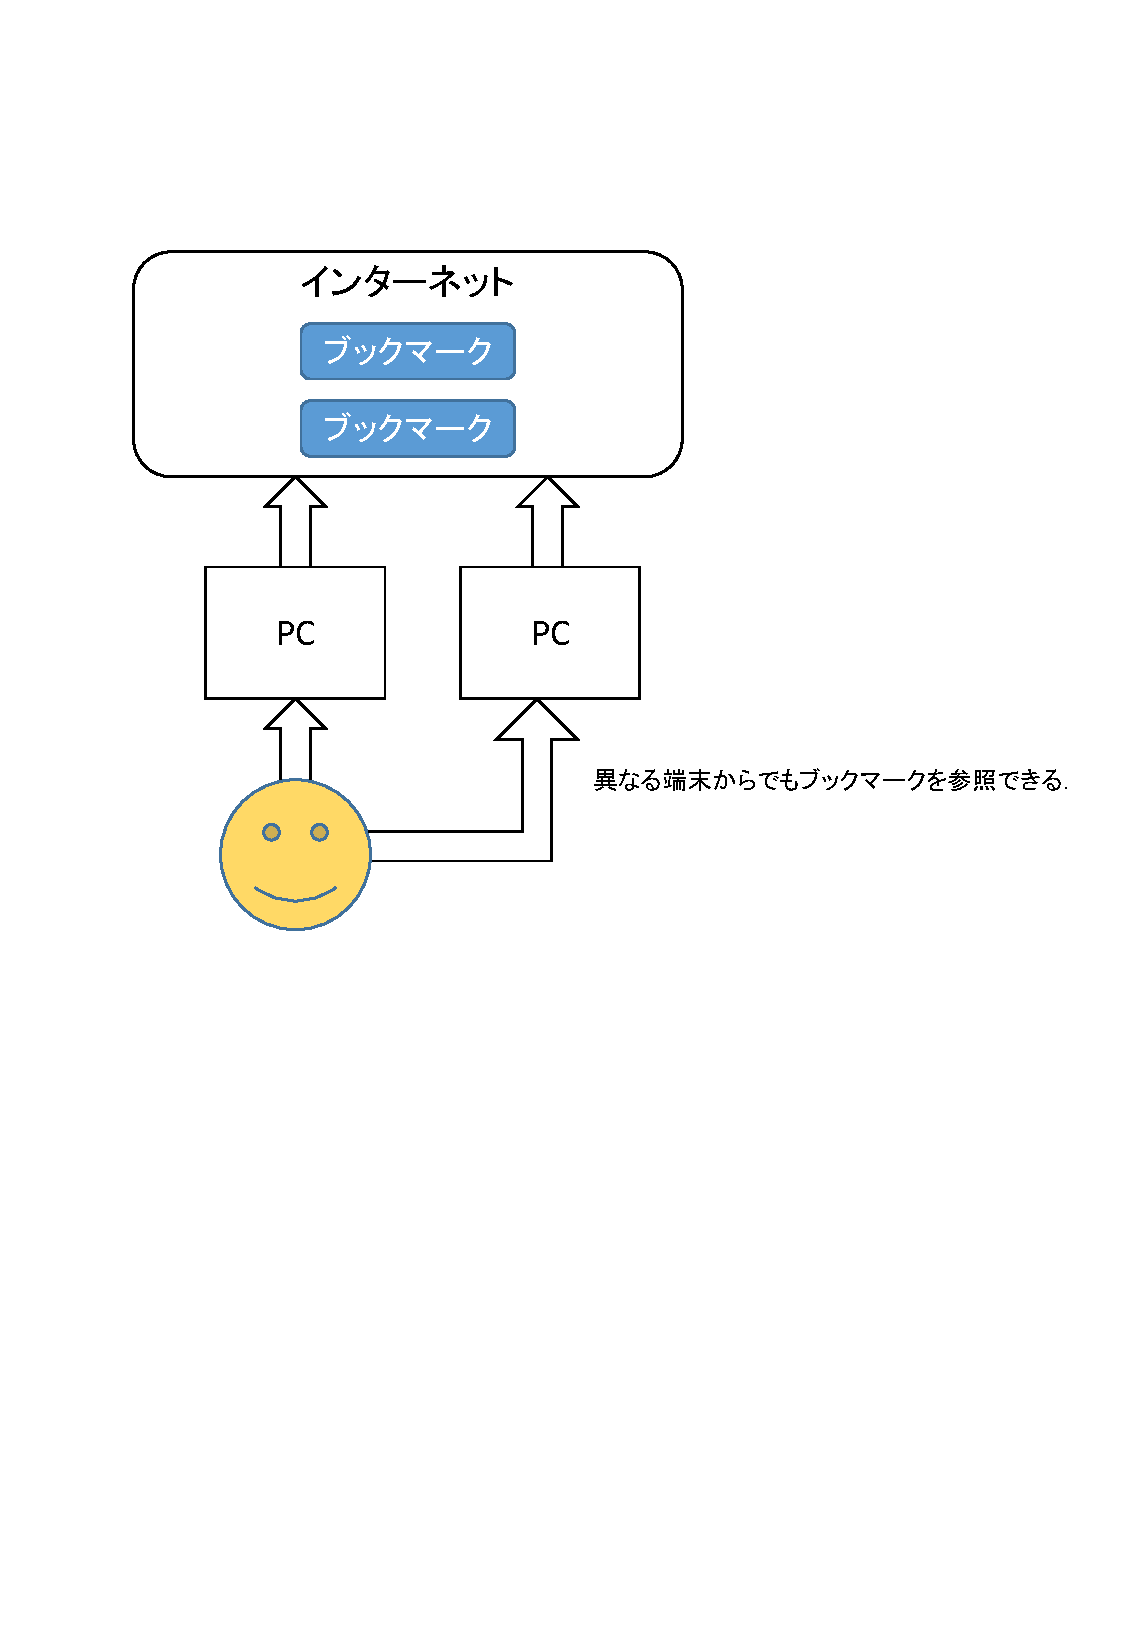
\includegraphics[width=10cm]{sbs1.pdf}
\caption{ソーシャルブックマーキングサービスのイメージ1}\label{sbs1}
\end{figure}

\newpage

また,他のユーザとブックマークを共有したり,タグをつけたり,コメントを残したりもできる.\par
自身のブックマークから推測し関心の持つ可能性の高いブックマークを発見しやすくなったり,注目のされているニュースなどを発見しやすくなる.
また様々なユーザが使用しているため様々なジャンルのブックマークを発見しやすくなる.

\begin{figure}[htb]
\centering
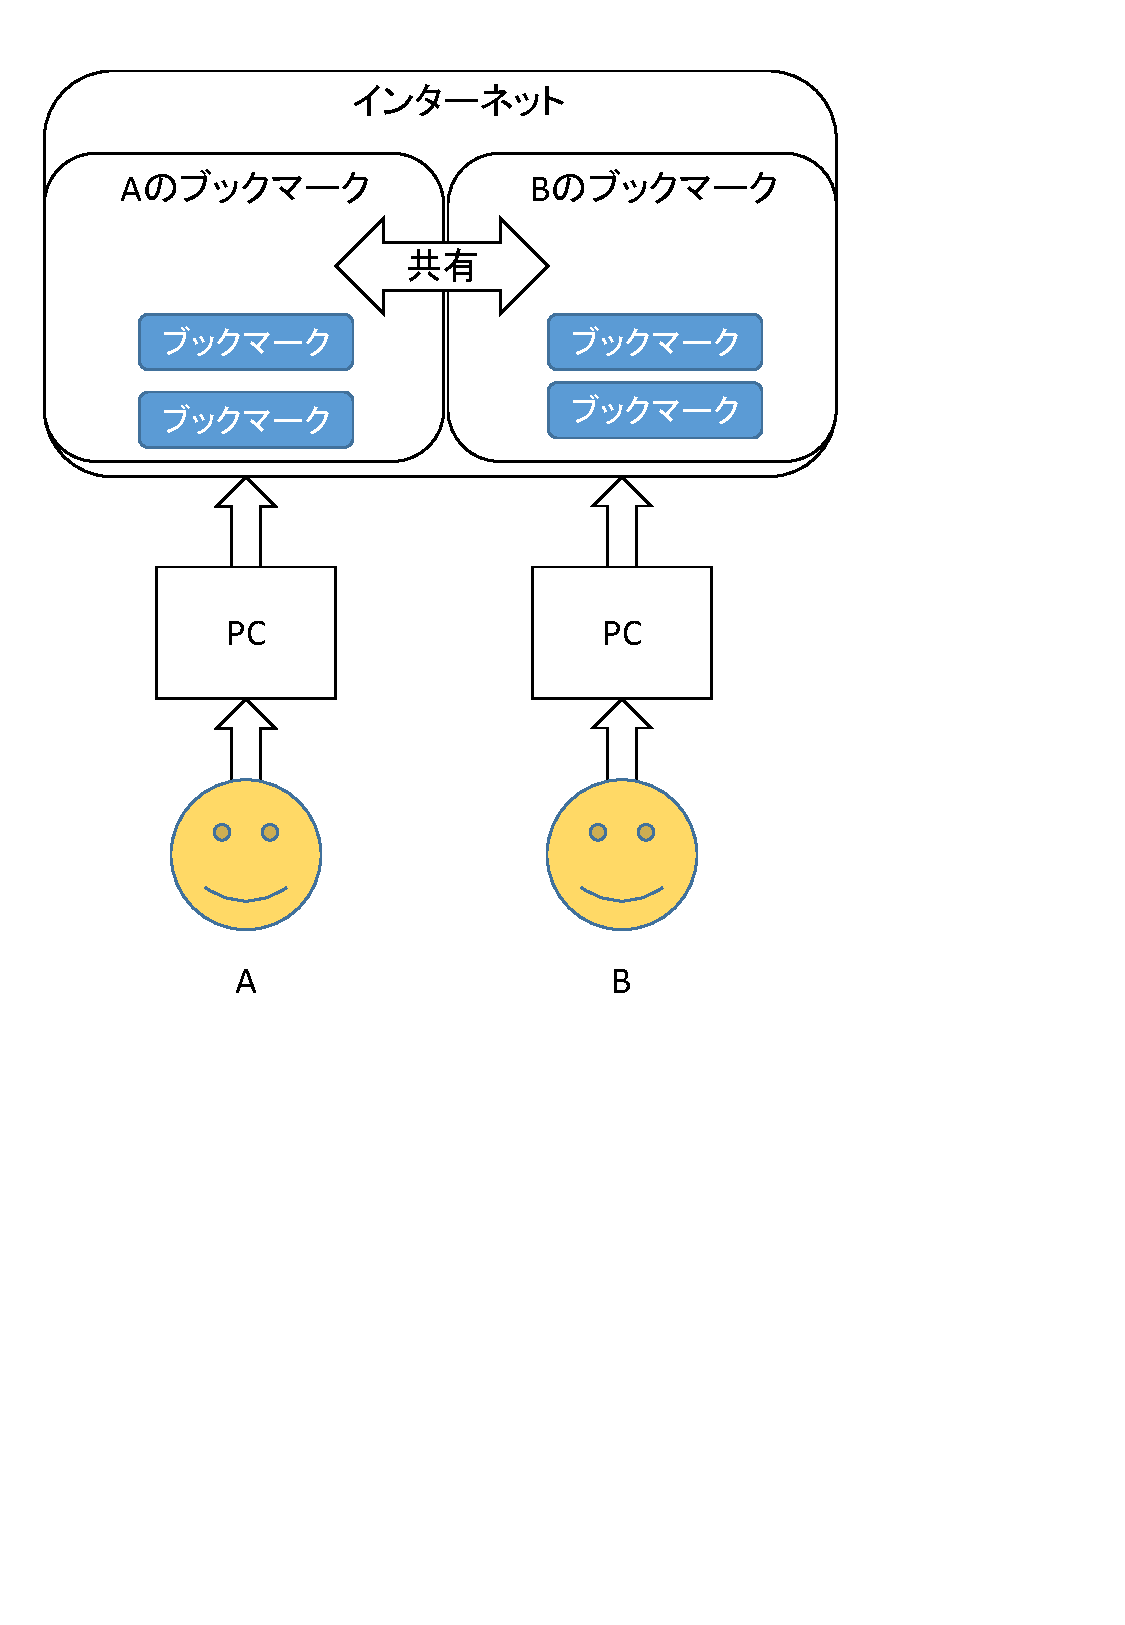
\includegraphics[width=10cm]{sbs2.pdf}
\caption{ソーシャルブックマーキングサービスのイメージ2}\label{sbs2}
\end{figure}

\chapter{はてなブックマークについて}
本章では本研究で使用するソーシャルブックマーキングサービスであるはてなブックマークについて解説する.

\section{はてなブックマークとは}
はてなブックマークとは,株式会社はてなの提供するソーシャルブックマーキングサービスである.\par
はてなブックマークは2005年2月にベータ版が開始され,同年8月に正式版が開始された\cite{hatena-history}.\par

\section{エントリとは}
はてなブックマークに登録されているブックマークのことをエントリという.\par
エントリは同じサイトをブックマークしている人がつけたタグやコメントを共有できる.

\newpage

\section{はてなブックマークの特徴}
株式会社はてなは,はてなブックマークの特徴として以下の3つの点を挙げている\cite{hatena-3}\cite{hatena-future}.

\subsection{保存}
端末を選ばないオンラインブックマーキングサービスと検索,タグ機能による情報の取り出しの容易さ.

\begin{enumerate}
\item オンラインにさえつながっていればいつでもブックマークを参照できる.
\item 様々な媒体でも共通のブックマークを参照できる.
\item 1000件以上のブックマークからでもタグなどの機能によって検索できる.
\end{enumerate}

\begin{figure}[htb]
\centering
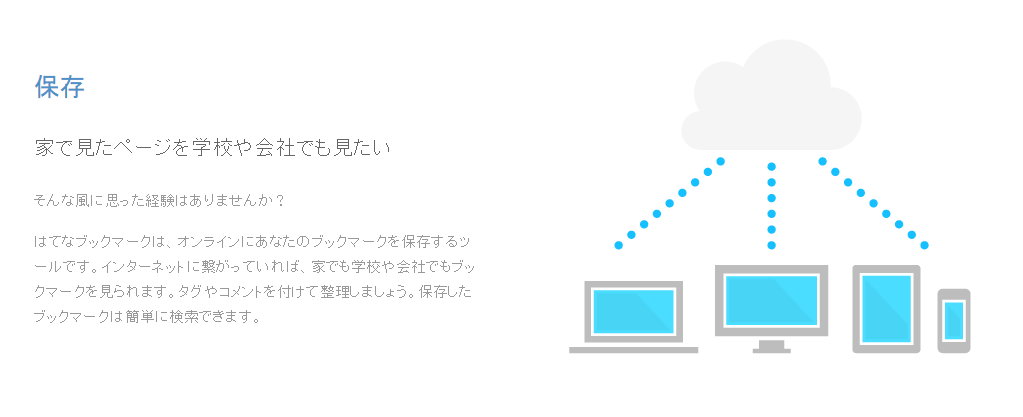
\includegraphics[width=13cm]{ho.PNG}
\caption{はてなブックマークの特徴1-保存}\label{hozon}
\end{figure}

\newpage


\subsection{共有}
ブックマークの公開による他のユーザーとのブックマークの共有ができる.


\begin{enumerate}
\item 公開されているほかの人のブックマークを参照できる.
\item 自身が広めたいと感じたブックマークは公開して共有できる.
\item コメントやタグをつけることで感想を共有できる.
\end{enumerate}


\begin{figure}[htb]
\centering
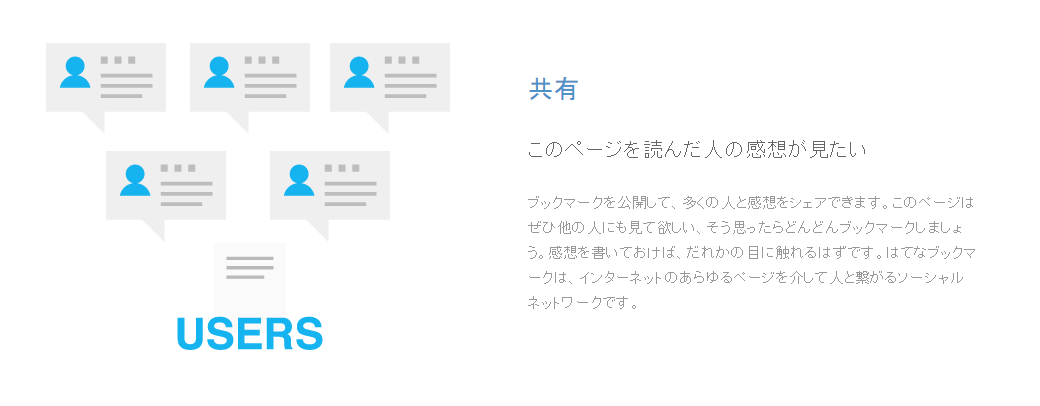
\includegraphics[width=13cm]{kyo.PNG}
\caption{はてなブックマークの特徴2-共有}\label{kyouyuu}
\end{figure}

\newpage

\subsection{発見}
人気エントリやキーワード検索などの機能によって情報の入手に幅ができる.


\begin{enumerate}
\item 人気エントリーや新着エントリーによって話題の情報が入手できる.
\item タグやキーワードで解く手のジャンルのみを検索できる.
\item 自分と似たユーザーをお気に入り登録すれば同じ趣味嗜好の情報を入手できる.
\end{enumerate}


\begin{figure}[htb]
\centering
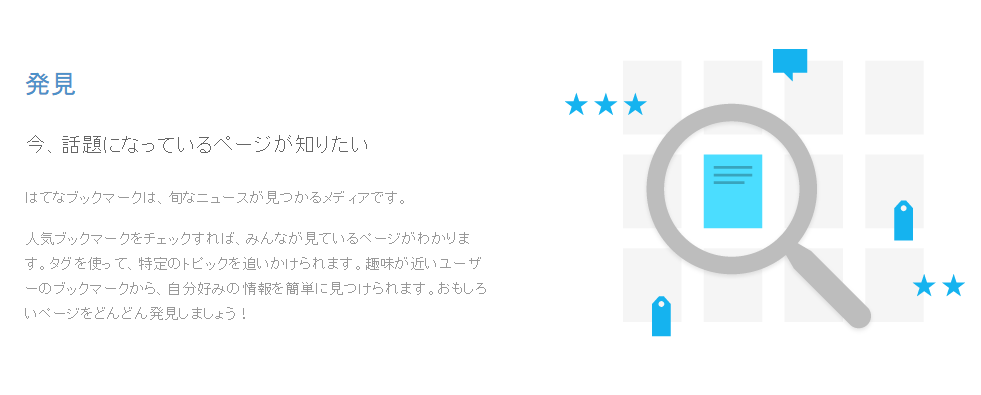
\includegraphics[width=13cm]{hak.PNG}
\caption{はてなブックマークの特徴3-発見}\label{hakken}
\end{figure}


\newpage

\section{株式会社はてな}
はてなブックマークを運営している株式会社はてなは2001年7月に有限会社はてなとして設立され,2004年2月に株式会社はてなに改組した\cite{hatena-history}.\par
人力検索はてなを始めとする様々なウェブサービスを提供している\cite{hatena-info}.\par

\section{はてなブックマークの選出理由}
ソーシャルブックマーキングサービスの中からはてなブックマークを選んだ理由を以下に挙げる.

\begin{enumerate}
\item 国内サービスの中では最大規模のソーシャルブックマーキングサービスであるため.
\item APIを公開してるため,データの収集が容易である.
\item コメントなどのが機能があるため収集できるデータが多い.
\end{enumerate}

\section{ホットエントリ}
ホットエントリとははてなブックマークで最近人気の勢いがあるブックマークである.\par
本研究ではこのホットエントリを取り扱い分析を進める.

\newpage

\section{はてなブックマークの利用方法と用語解説}
はてなブックマークの画面について解説する.

\subsection{はてなブックマークのトップ画面}
この画面では多くのユーザーに共有されているブックマークが表示される.

\begin{figure}[htb]
\centering
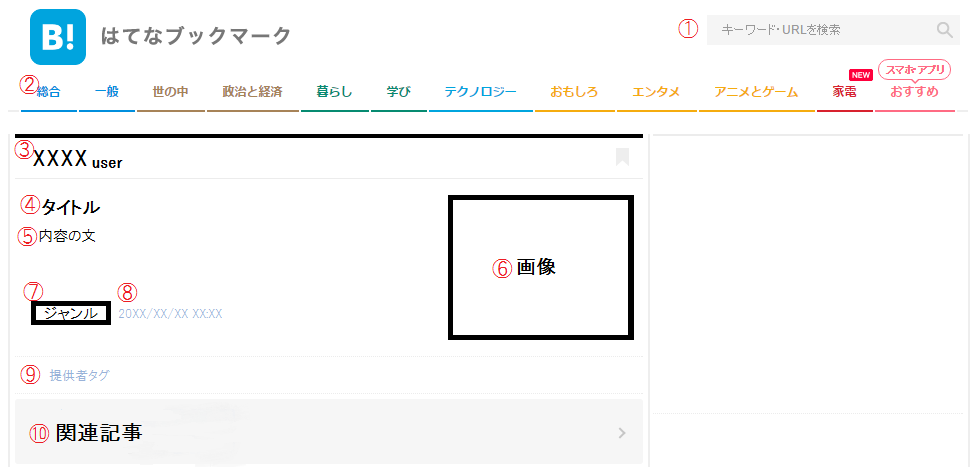
\includegraphics[width=15cm]{hatena-1.png}
\caption{ブックマーク一覧での表示}\label{hatenatop}
\end{figure}

\subsubsection{検索ウィンドウ(図4.1‐1)}
ここにキーワードを打つことでその言葉に関連するブックマークを検索することができる.\par
図4.2はその結果である.
\subsubsection{ジャンル一覧(図4.1‐2)}
はてなブックマークでのジャンル一覧であり,ジャンルの名前をクリックすることでブックマークをジャンルごとに表示させる.
\subsubsection{ユーザー数(図4.1‐3)}
そのブックマークを共有しているユーザー数である.クリックすることで詳細画面へ行く.
\subsubsection{タイトル(図4.1‐4)}
そのブックマークのタイトルである.クリックすることでそのブックマークのサイトへ行く.
\subsubsection{内容(図4.1‐5)}
そのブックマークの内容を表示する.表示しきれない場合は省略される.
\subsubsection{画像(図4.1‐6)}
そのブックマークにある画像が表示される.画像がない場合は表示されずそのスペースに内容が表示される.
\subsubsection{ジャンル(図4.1‐7)}
そのブックマークが分類されているジャンルが表示される.クリックすることでそのジャンルが表示される.
\subsubsection{掲載日時(図4.1‐8)}
そのブックマークが掲載された時間である.
\subsubsection{提供者タグ(図4.1‐9)}
そのブックマークのエントリを提供しているサイトのタグである.クリックすることでそのサイトの関連エントリが表示される.エントリとははてなブックマークで登録されているブックマークのことである.
\subsubsection{関連エントリ(図4.1‐10)}
そのエントリに関連付けられたブックマークがある場合表示される.
関連がない場合は表示されない.

\newpage

\subsection{はてなブックマークでの記事検索画面}
この画面では検索したワードにヒットしたブックマークが表示される.

\begin{figure}[htb]
\centering
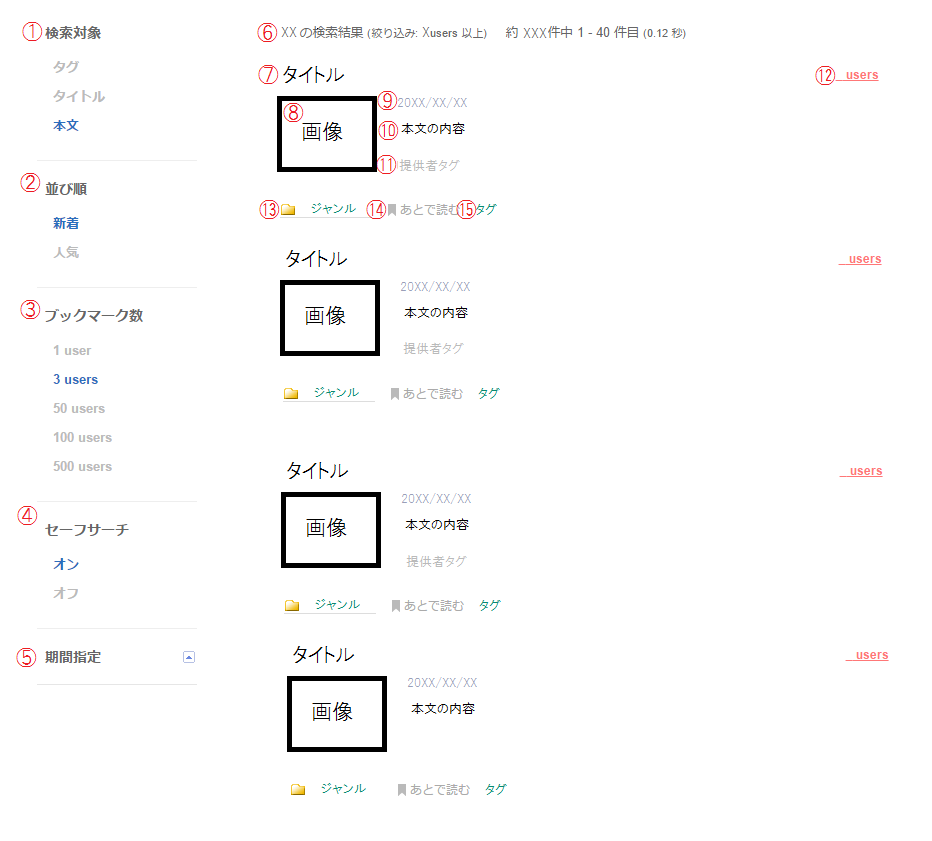
\includegraphics[width=15cm]{hatena-3.png}
\caption{ブックマークの検索結果}\label{hatenasearch}
\end{figure}

\subsubsection{検索対象設定(図4.2‐1)}
検索ワードの対象を設定する.タグ,タイトル,本文の3つから選択できる.
\subsubsection{並び順(図4.2‐2)}
検索結果のソートを行う.時間と登録数でソートが行える.
\subsubsection{ブックマーク数絞り込み(図4.2‐3)}
ブックマーク数による絞り込みを行う.クリックした数以上のブックマークを表示する.1,3,50,100,500の数値で絞り込みが行える.
\subsubsection{セーフサーチ(図4.2‐4)}
検索結果にフィルターをかける.オンにした場合検索結果から不適切な表現がある記事を除外する.
\subsubsection{期間指定(図4.2‐5)}
表示するブックマークの掲載された期間の指定をする.
プルダウンを押下すると期間指定のための入力ウィンドウが2つ表示される.1つ目の入力ウィンドウから2つ目の入力ウィンドウの間の期間が表示される.
\subsubsection{検索結果のヒット数(図4.2‐6)}
検索した結果,該当したブックマークの数が表示される.
\subsubsection{タイトル(図4.2‐7)}
検索にヒットしたブックマークのタイトルである.検索したワードがタイトルに含まれている場合,その部分がハイライトされる.クリックすることでブックマークのサイトが表示される.
\subsubsection{画像(図4.2‐8)}
そのブックマークにある画像が表示される.画像がない場合は表示されずそのスペースに内容が表示される.
\subsubsection{掲載日時(図4.2‐9)}
そのブックマークが掲載された時間である.期間指定をした場合この数値を参照する.
\subsubsection{内容(図4.2‐10)}
そのブックマークの内容を表示する.表示しきれない場合は省略される.
\subsubsection{提供者タグ(図4.2‐11)}
そのブックマークの記事を提供しているサイトのタグである.クリックすることでそのサイトの関連記事が表示される.
\subsubsection{ユーザー数(図4.2‐12)}
そのブックマークを共有しているユーザー数である.クリックすることで詳細画面へ行く.
\subsubsection{ジャンル(図4.2‐13)}
そのブックマークが分類されているジャンルが表示される.クリックすることでそのジャンルが表示される.
\subsubsection{あとで読む(図4.2‐14)}
そのブックマークに後で読むタグをつけ,未読の場合通知する.
\subsubsection{タグ(図4.2‐15)}
そのブックマークにつけられたタグを表示する.タグ検索ではここを参照する.タグをクリックすると同じタグをもつブックマークを表示する.

\newpage

\subsection{ブックマーク記事の詳細}
この画面ではブックマークの詳細を見ることができる.

\begin{figure}[htb]
\centering
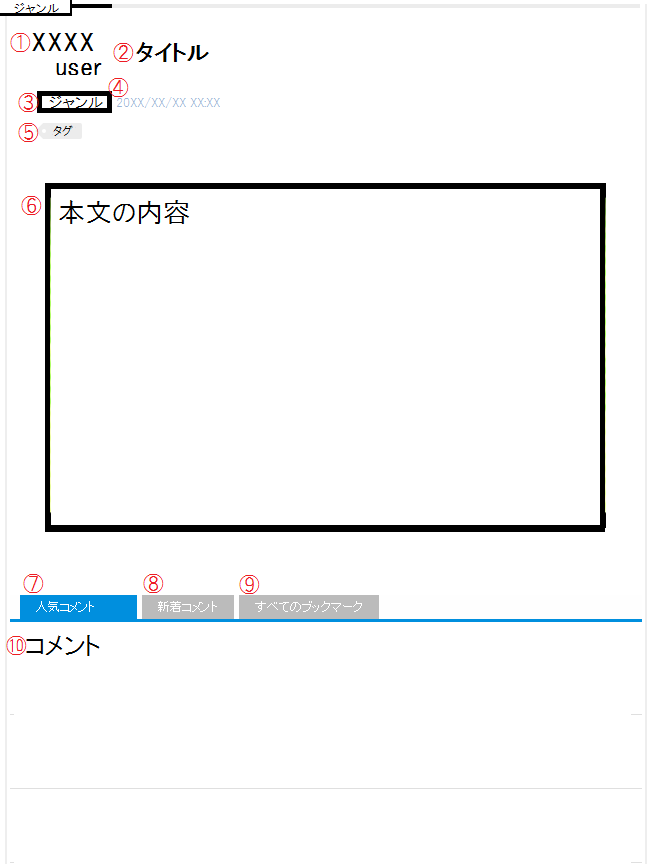
\includegraphics[width=13cm]{hatena-2.png}
\caption{ブックマークの詳細表示}\label{hatena-info}
\end{figure}

\subsubsection{ユーザー数(図4.3‐1)}
そのブックマークを共有しているユーザー数である.
\subsubsection{タイトル(図4.3‐2)}
そのブックマークのタイトルである.クリックすることでそのブックマークのサイトへ行く.
\subsubsection{ジャンル(図4.3‐3)}
そのブックマークが分類されているジャンルが表示される.クリックすることでそのジャンルが表示される.
\subsubsection{掲載日時(図4.3‐4)}
そのブックマークが掲載された時間である.
\subsubsection{タグ(図4.3‐5)}
そのブックマークにつけられたタグを表示する.タグをクリックすると同じタグをもつブックマークを表示する.
\subsubsection{内容(図4.3‐6)}
そのブックマークの内容を表示する.動画などの場合はここで再生もできる.
\subsubsection{人気コメント(図4.3‐7)}
コメント欄に表示するコメントを多くスターを集めているものだけにする.
\subsubsection{新着コメント(図4.3‐8)}
コメント欄に表示するコメントを新着順にする.
\subsubsection{すべてのブックマーク(図4.3‐9)}
コメントの有無にかかわらずこのエントリをブックマークしたユーザを表示する.
\subsubsection{コメント欄(図4.3‐10)}
図4.2‐7.8.9の押したものによってそれに合うコメントを表示する.

\newpage


\chapter{研究環境の構築}
本研究を進める上での環境を解説する.

\section{Virtual Boxのインストール}
本研究を進めるためのプログラムを起動する仮想マシンの構築を行う.
\subsection{Virtual Boxとは}
仮想マシンの構築,管理を行うソフトである.仮想マシン上ではホストとは異なる環境を構築することも可能であり,様々な作業を仮想マシン上で行うことが可能である\cite{vb}.

\newpage

\subsection{Chocolateyのインストール}
Virtual BoxをインストールするためにまずChocolateyをインストールする.

コマンドプロンプトを開き,以下の画像のコマンドを実行する.

\begin{figure}[htb]
\centering
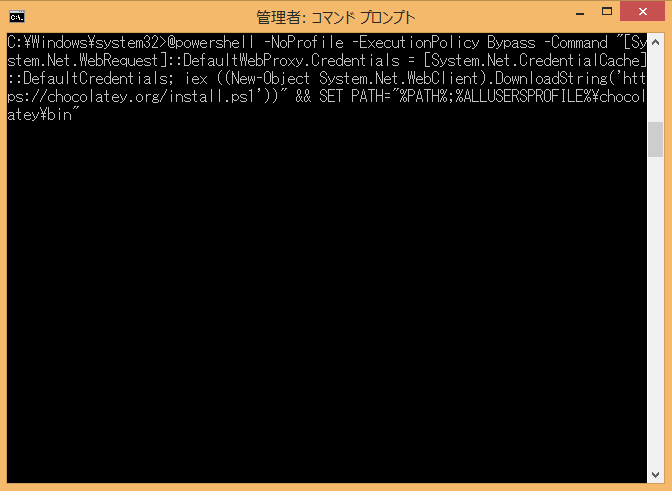
\includegraphics[width=15cm]{choco-cmd1.png}
\caption{Chacolateyのインストール画面}\label{chocoinst}
\end{figure}

\newpage

以下の画像のようになったら成功である.

\begin{figure}[htb]
\centering
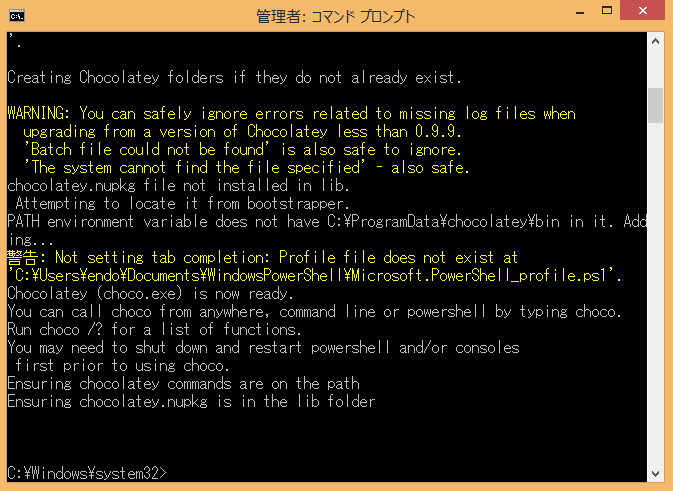
\includegraphics[width=15cm]{choco-cmd2.png}
\caption{Chacolateyのインストール画面2}\label{chocoinst2}
\end{figure}

\newpage

\section{Virtual Boxのインストール}
コマンドプロンプトを開き,以下の画像のコマンドを入力する.

\begin{figure}[htb]
\centering
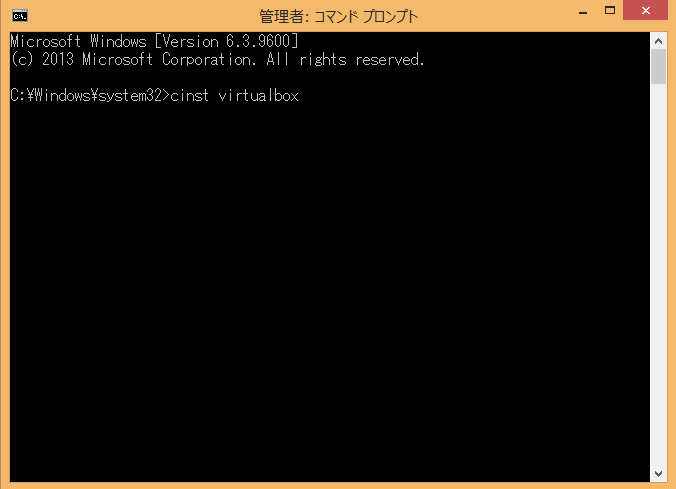
\includegraphics[width=15cm]{vb-cmd1.png}
\caption{Virtual Boxのインストール画面}\label{vbinst1}
\end{figure}

\newpage
ここでYを入力しEnterを押す.

\begin{figure}[htb]
\centering
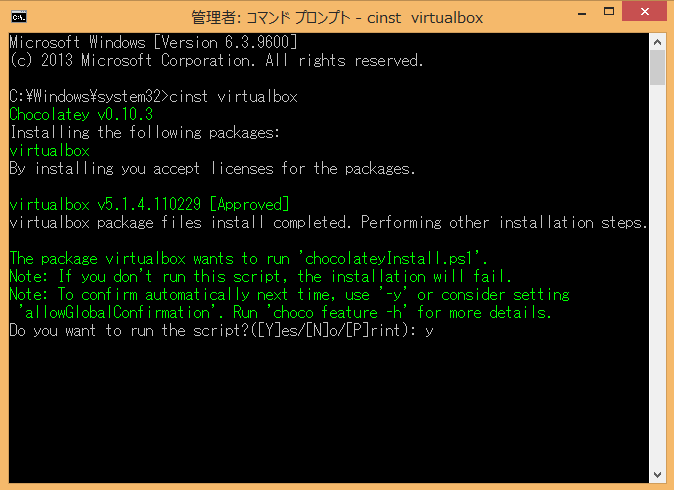
\includegraphics[width=15cm]{vb-cmd2.png}
\caption{Virtual Boxのインストール画面2}\label{vbinst2}
\end{figure}

\newpage


以下の画像のようになったら成功である.

\begin{figure}[htb]
\centering
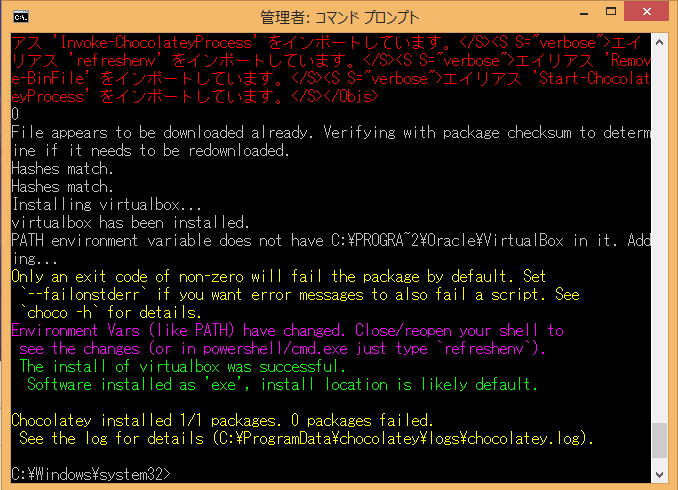
\includegraphics[width=15cm]{vb-cmd3.png}
\caption{Virtual Boxのインストール画面3}\label{vbinst3}
\end{figure}

\newpage

\section{計算機環境の構築}

\subsection{計算機環境の導入}
本研究には矢吹研究室にて構築した計算機環境をクローンして使用する.
\begin{figure}[htb]
\centering
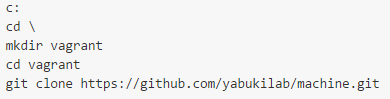
\includegraphics[width=13cm]{cl.PNG}
\caption{導入コマンド}\label{clone}
\end{figure}

\subsection{コマンド}
基本的なコマンドを以下に記す.


\subsubsection{vagrant up}
仮想マシンの起動を行う.
\subsubsection{vagrant ssh}
仮想マシンの再起動を行う.
\subsubsection{vagrant halt}
仮想マシンの停止を行う.
\subsubsection{vagrant destroy}
仮想マシンの削除を行う.


\chapter{目的}

ソーシャルブックマーキングサービスにおけるサイトのブックマーク数の推移を調査し分析することで,ブックマーク数の増加傾向や伸びやすい時間帯の分析を行う.\par
その結果をもとに考察を行い,増加傾向のパターンの可視化及び分類をする.それによりウェブマーケティングを行う上での指標の一つを作成することを目的とする.

\chapter{手法}
本研究ではソーシャルブックマーキングサービスの1つであるはてなブックマークを使用しデータを収集する.

\section{データの収集方法}
はてなブックマークのAPI\cite{hatena-develop}を使用し,はてなブックマークのトップ画面からエントリ情報を収集する.\par
はてなブックマークのAPI用のURLの後ろに対象のURLを記載することで対象のエントリの各データをjson形式で取得できる.

\begin{figure}[htb]
\centering
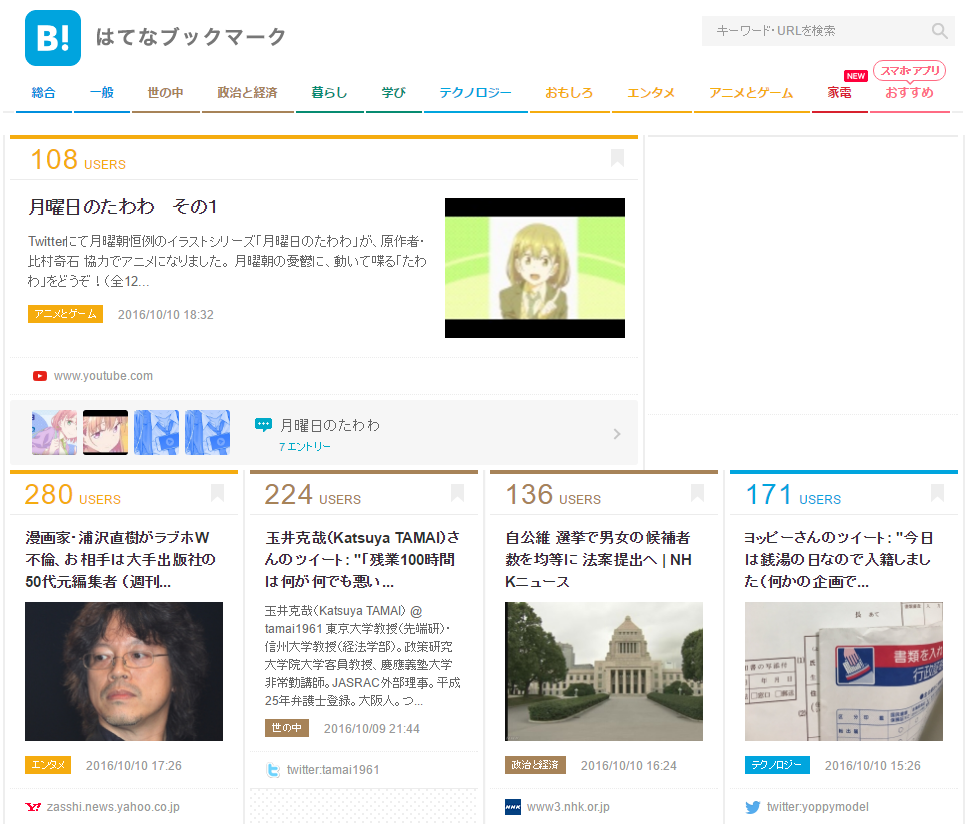
\includegraphics[width=10cm]{hatena-ta.png}
\caption{はてなブックマークトップ画面}\label{hatenatop}
\end{figure}

\newpage

\section{APIによるデータの収集範囲}
はてなブックマークのトップページの人気のエントリ100件を対象に,はてなブックマークのAPI\cite{hatena-api}を使用しデータを取得する.
APIを使用することにより対象エントリに含まれるデータが取得できる.
以下に取得できるデータの種類を列挙する.\par

\subsection{取得できる対象エントリのデータ一覧}

\begin{enumerate}
\item title
\item count 
\item url
\item entry-url
\item screenshot
\item eid 
\item bookmarks ユーザーが対象エントリに行ったブックマークごとの詳細である.
\item related 対象エントリに関連の深いエントリのデータである.
\end{enumerate}

\subsection{取得データの詳細}
対象エントリ取得した8種のデータのうちbookmarksとrelatedに関しては複数の要素を含む.
以下にその種類を列挙する.

\subsubsection{bookmarks}

\begin{enumerate}
\item user 
\item tags
\item timestamp 
\item comment
\end{enumerate}

\subsubsection{related}

\begin{enumerate}
\item title
\item url
\item entry-url
\item eid
\end{enumerate}

\newpage

\section{APIを利用したデータ取得プログラム}
はてなブックマークのAPIを利用し,エントリデータを取得するプログラムを作成した.\par
以下に作成したプログラムの画像とその一連の流れの説明である.

\begin{figure}[htb]
\centering
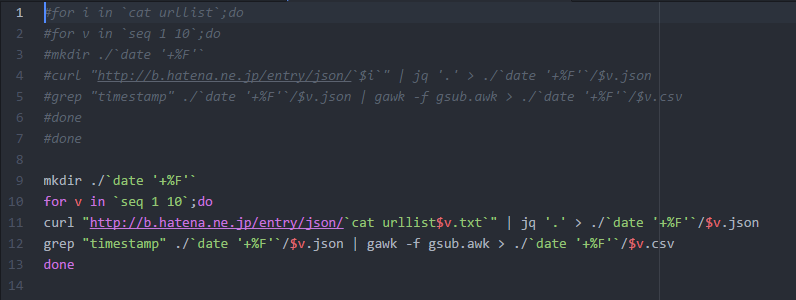
\includegraphics[width=13cm]{sh.PNG}
\caption{データ取得プログラム}\label{sh}
\end{figure}
事前にurllistというtxtファイルを作っておき,そこに対象のエントリのもとのページのURLを格納しておく.\par
curlによって対象のURLの前にはてなブックマークのAPIを接続し,取得したデータをJQueryで整理し,json形式で出力する.\par
grepによってtimestampを抽出し,awkによって時間データのみに置換する.その後csv形式に日付データを出力する.


\newpage

\section{JQueryによる取得したデータの整理}
APIによって取得したデータのJQueryによる処理の説明について記す.

\subsection{データの整理}
はてなブックマークのAPIで取得したデータはjson形式で保存される.json形式は整理を行わなくては閲覧が難しいためデータの整理を行い,閲覧の可能な状態にする必要がある.\par
データの整理にはJQueryを使用する.

\subsection{JQueryについて}
Javascriptのライブラリの一つであり,今回はjson形式のファイルの整理に使用する.

\subsection{整理の実行}
取得したjson形式のデータにJQueryを実行することで閲覧可能な状態に整理することができる.


\newpage

\subsection{json形式のデータの構造}
以下にはてなブックマークのAPIを使用して取得したjson形式のデータの構造を記す.

\subsubsection{エントリの基本情報}
jsonの上部に記載されているエントリの基本情報である.

\begin{figure}[htb]
\centering
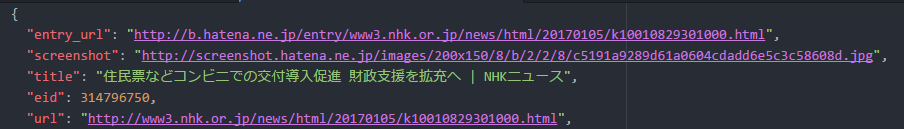
\includegraphics[width=13cm]{json1.PNG}
\caption{json形式のファイルの構造例1}\label{json1}
\end{figure}

\subsubsection{entry-url}
はてなブックマーク内での対象エントリの概要ページのURLである.\par
http://b.hatena.ne.jp/entry/...の形式で表示される.
\subsubsection{screenshot}
対象エントリのスクリーンショットのURLである.画像はjpg形式となる.  \par
http://screenshot.hatena.ne.jp/images/...の形式で表示される.
\subsubsection{title}
対象エントリのタイトルである.
\subsubsection{eid}
内部でふられている対象エントリのIDである.\par
9桁の数字が羅列される.
\subsubsection{url}
対象エントリのもとのページのURLである.

\newpage

\subsection{エントリのブックマーク情報}
bookmarksは基本情報の下に記録されているブックマークの情報の一覧である.\par
bookmarksには4種類のデータが含まれる.

\begin{figure}[htb]
\centering
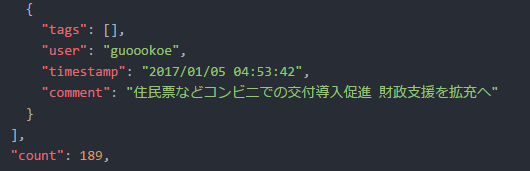
\includegraphics[width=13cm]{json2.PNG}
\caption{json形式のファイルの構造例2}\label{json2}
\end{figure}

\subsubsection{tags}
対象エントリにユーザーがつけたユーザーごとのタグである.\par
複数ある場合はそのすべてが列挙される.
\subsubsection{user}
対象エントリをブックマークしたユーザーの名前である.
\subsubsection{timestamp}
対象エントリがブックマークされた時間の記録である.\par
西暦/月/日 時:分:秒の形式で表記される.
\subsubsection{comment}
対象エントリのブックマークにつけられたコメントの内容である.
\subsubsection{count}
対象エントリをブックマークした合計人数である.

\newpage
\subsection{エントリに関連の深いエントリ情報}
relatedはブックマーク情報の下に記録されている関連エントリの情報である.
relatedには種類のデータが含まれる.

\begin{figure}[htb]
\centering
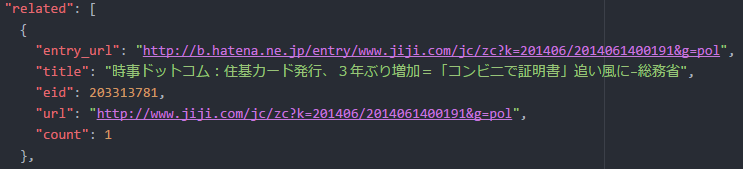
\includegraphics[width=13cm]{json3.PNG}
\caption{json形式のファイルの構造例3}\label{json2}
\end{figure}

\subsubsection{entry-url}
はてなブックマーク内での関連エントリの概要ページのURLである.
http://b.hatena.ne.jp/entry/...の形式で表示される.
\subsubsection{title}
関連エントリのタイトルである.
\subsubsection{eid}
内部でふられている関連エントリのIDである.
9桁の数字が羅列される.
\subsubsection{url}
関連エントリのもとのページのURLである.
\subsubsection{count}
関連対象エントリをブックマークした合計人数である.エントリをブックマークした合計人数である.

\newpage

\subsection{その他のデータの記録}
研究における参考やデータの整理のために使用するデータを以下に記す.

\subsubsection{記録日時}
処理のため各エントリにつける番号である.
\subsubsection{通し番号}
対象エントリのデータを取得した時間である.
\subsubsection{ジャンル}
対象エントリがはてなブックマークで分類されているジャンルの種類である.

\newpage

\section{取得したデータの抽出}
はてなブックマークのAPIによって取得したデータから本研究に使用する要素のみを抽出する.
抽出にはgrepを使用する.また余分データの置換にはawkを使用する.
以下に処理の手順について解説する.

\subsection{grepとは}
linuxコマンドの一つで文字列の検索,抽出を行えるコマンドである.

\subsection{awkとは}
unixで開発されたプログラム言語であり,テキストファイルの処理を行える.\par
区切りのあるデータの処理を特に得意とする.

\subsubsection{JQueryによるデータの整理}
jsonファイルを整理し,閲覧可能な状態にしている.\par
以下に画像はJQueryによって閲覧が可能となったデータである.
\begin{figure}[htb]
\centering
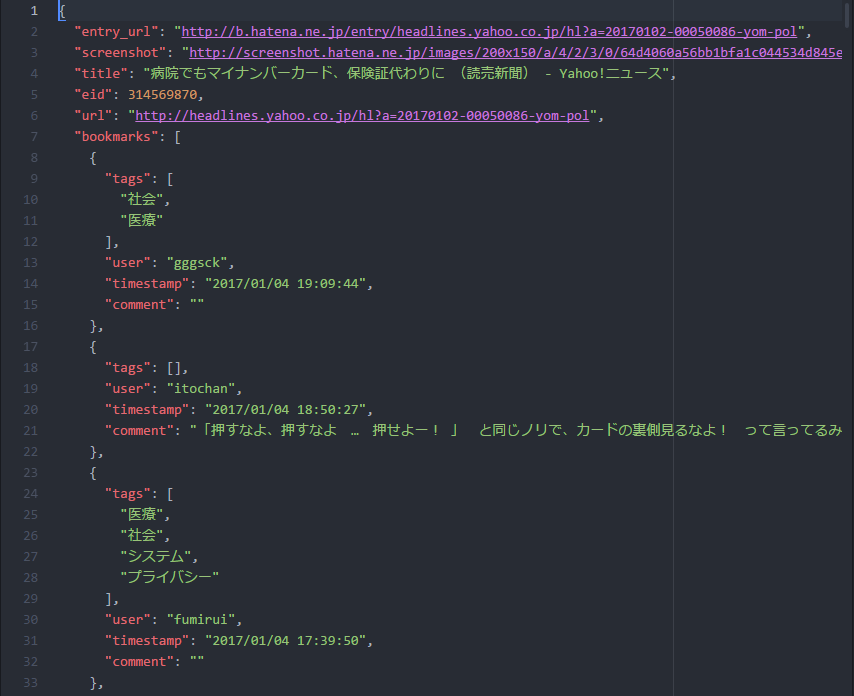
\includegraphics[width=10cm]{jq.PNG}
\caption{JQueryによる整理の結果}\label{jq}
\end{figure}

\newpage

\subsubsection{grepによるデータの抽出}
grepで抽出したブックマークの時間データは以下の画像のようになる.

\begin{figure}[htb]
\centering
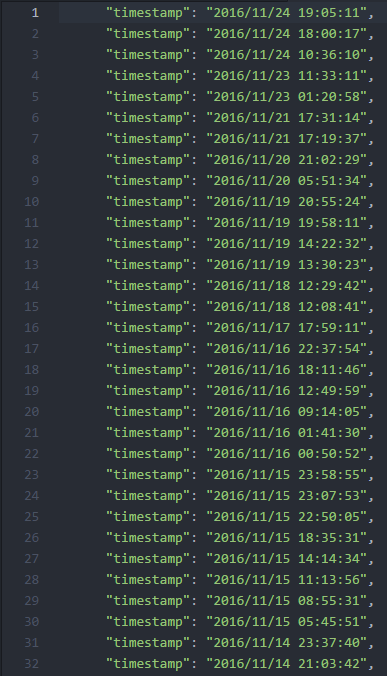
\includegraphics[width=10cm]{timestamps.PNG}
\caption{grepによる時間データの抽出}\label{excel7}
\end{figure}

\newpage

\subsubsection{awkによる余分データの置換}
余分データを置換することで時間データのみの抽出を行う.\par
以下の画像は今回処理に用いたawkである.

\begin{figure}[htb]
\centering
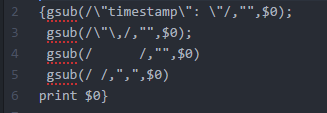
\includegraphics[width=13cm]{gsub.PNG}
\caption{実行したawk}\label{g3}
\end{figure}

\newpage

また,以下の画像は時間データのみを抽出した結果である.

\begin{figure}[htb]
\centering
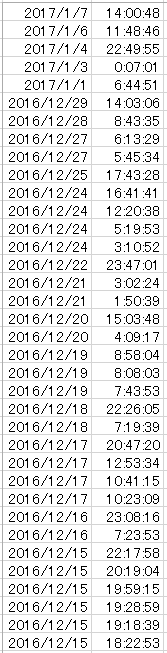
\includegraphics[width=4.5cm]{awk.PNG}
\caption{awkによる余分データの置換結果}\label{awk}
\end{figure}

\newpage

\section{取得したデータの処理}
はてなブックマークのAPIを使用し取得したデータを分析するために行う処理について記載する.
以下の一連の作業をマクロとして記録し,処理を行う.

\subsection{データの変換}
はてなブックマークを使用して取得したjson形式のデータをcsv形式に変換し出力する.
csv形式で出力されたデータは以下のようになる.

\begin{figure}[htb]
\centering
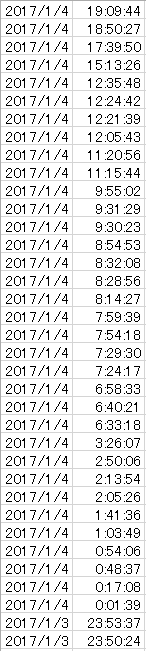
\includegraphics[width=3cm]{excel1.PNG}
\caption{csv形式での出力結果}\label{excel1}
\end{figure}

\newpage

\subsection{データの統合}
csv形での出力では初期状態では日付と時刻が同一セルに存在していないため,それらを統合する必要がある.\par
excelでは日付及び時刻を数値に変換した場合,自然数部分が日付にあたり,小数点以下が時刻にあたる.
そのため日付と時刻に対し加算を行えば統合することができる.\par
以下の画像は時間データの統合結果である.

\begin{figure}[htb]
\centering
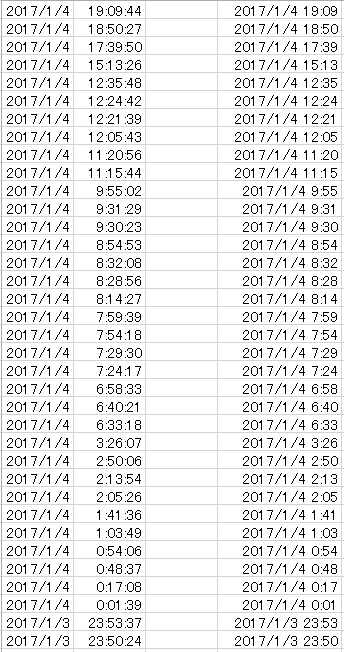
\includegraphics[width=6cm]{excel2.PNG}
\caption{日付と時刻の統合結果}\label{excel2}
\end{figure}

\newpage

\subsection{番号の振り分け}
json形式では日付の新しい順でデータが並べられているので,ブックマーク数の増加の推移を可視化するにあたり昇順でデータのソートを行う.\par
ソート後,時間データに番号をふる.\par
以下の画像は日付データのソート結果と番号の振り分けの結果である.

\begin{figure}[htb]
\centering
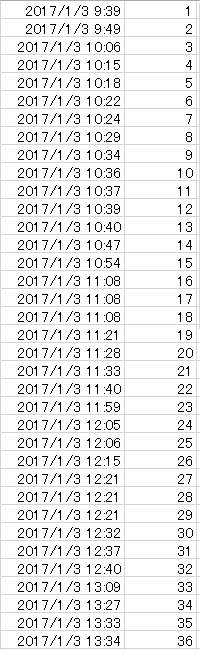
\includegraphics[width=5cm]{excel3.PNG}
\caption{データのソート結果及び番号の振り分け}\label{excel3}
\end{figure}

\newpage

\section{時間の推移とブックマーク数の増加の推移の可視化}
縦軸にブックマーク数と横軸に日付データを設定し,時間の推移におけるブックマーク数の増加の傾向に関して散布図を作成し可視化する.\par
以下の画像は時間の推移におけるブックマーク数の増加の傾向を可視化した結果の例である.

\begin{figure}[htb]
\centering
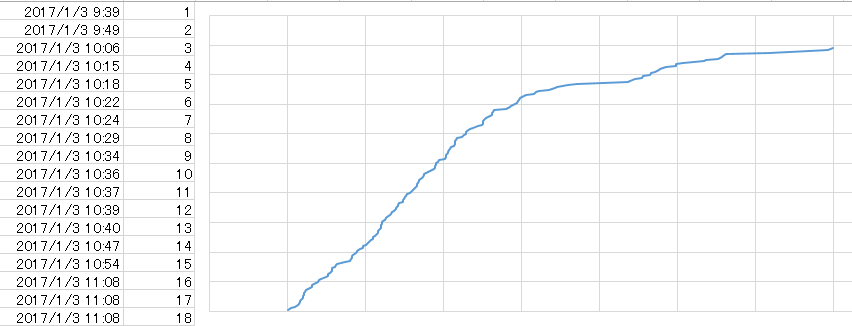
\includegraphics[width=13cm]{excel4.PNG}
\caption{時間の推移とブックマーク数の増加の推移の可視化の結果}\label{excel4}
\end{figure}

\newpage

\section{時間経過によるブックマーク数の増加}
初めてエントリがブックマークがされてから6時間ごとのブックマーク数増加数を算出する.

\begin{figure}[htb]
\centering
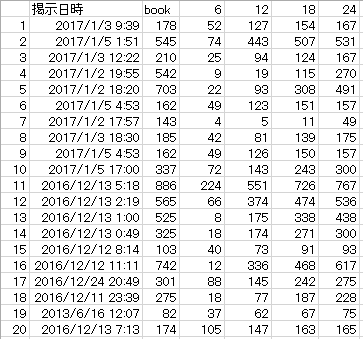
\includegraphics[width=8cm]{excel5.PNG}
\caption{時間経過によるエントリのブックマークの増加数}\label{excel5}
\end{figure}

\newpage

\section{時刻ごとのブックマーク数の増加}
初めてエントリがブックマークがされてから24時間以内を対象に1時間ごとの時刻のブックマーク数の増加数を算出する.


\subsection{時間データの変換}
各時刻ごとの増加数を求めるため時間データを処理できる数値に変換する.\par
数値に変換した際,自然数部分が日付にあたり,小数点以下が時刻を表している.ここでは各時刻ごとの増加数を求めるため,小数点以下の数値のみを抽出する.\par
時刻データの抽出はINT関数を使用する.
以下は数値データへの変換と時刻データの抽出の結果である.
左部が元データ,中央部が数値変換の結果,右部が抽出した時刻データである.

\begin{figure}[htb]
\centering
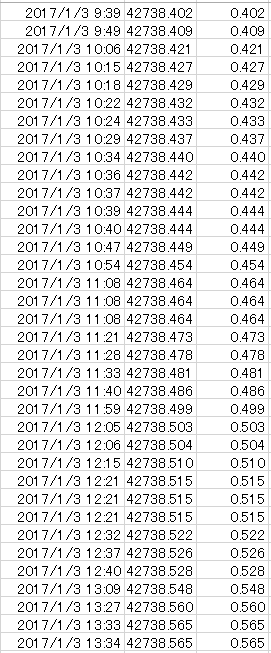
\includegraphics[width=5cm]{excel6.PNG}
\caption{数値への変換と時刻データの抽出}\label{excel6}
\end{figure}

\newpage

\subsection{時刻ごとの増加数のカウント}
次に時刻ごとのブックマーク数の増加数を算出する.\par
1日を1として扱い,24時間ごとの数値にすると1時間当たり0.04166...となる.
よって各時刻の増加数を算出するにはCOUNTIFS関数を使用し,各時刻ごとに条件付けし,該当する数をカウントする.\par
各時刻ごとの条件は対象の時刻をxとし,0.041667にxをかけ,0.041667x以上0.041667(x+1)未満に該当する数とすることで対象の時刻の増加数が算出できる.\par

\begin{figure}[htb]
\centering
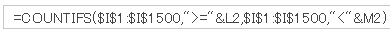
\includegraphics[width=13cm]{countifs.PNG}
\caption{countifs関数}\label{count}
\end{figure}

\newpage

以下はあるエントリの各時刻ごとのブックマークの増加数である.\par
左部は時刻,中央部は条件数値,右部は増加数である.

\begin{figure}[htb]
\centering
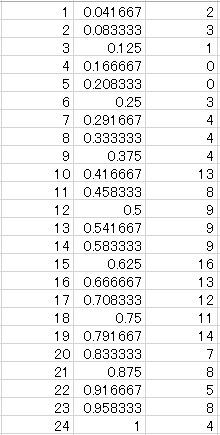
\includegraphics[width=8cm]{excel7.PNG}
\caption{各時刻ごとの条件数値と増加数}\label{excel7}
\end{figure}


\section{分析}
時間の推移に伴うブックマーク数の増加について可視化を行い,その増加の傾向からパターン分けを行う.\par


\chapter{結果}
100件のデータに対し,3種類の分析を行った.
\section{時間の推移に伴うブックマーク数の増加の傾向のパターン}
時間の推移に伴うブックマーク数の増加について可視化を行ったところ大きく分けて3つのパターンに分類することができた.\par
以下に分類した推移のパターンと解説を記す.

\subsection{平均型}
安定してブックマーク数が伸び続ける.急な上昇や大きな衰退もなく,ほぼ直線に近い推移を見せる.

\begin{figure}[htb]
\centering
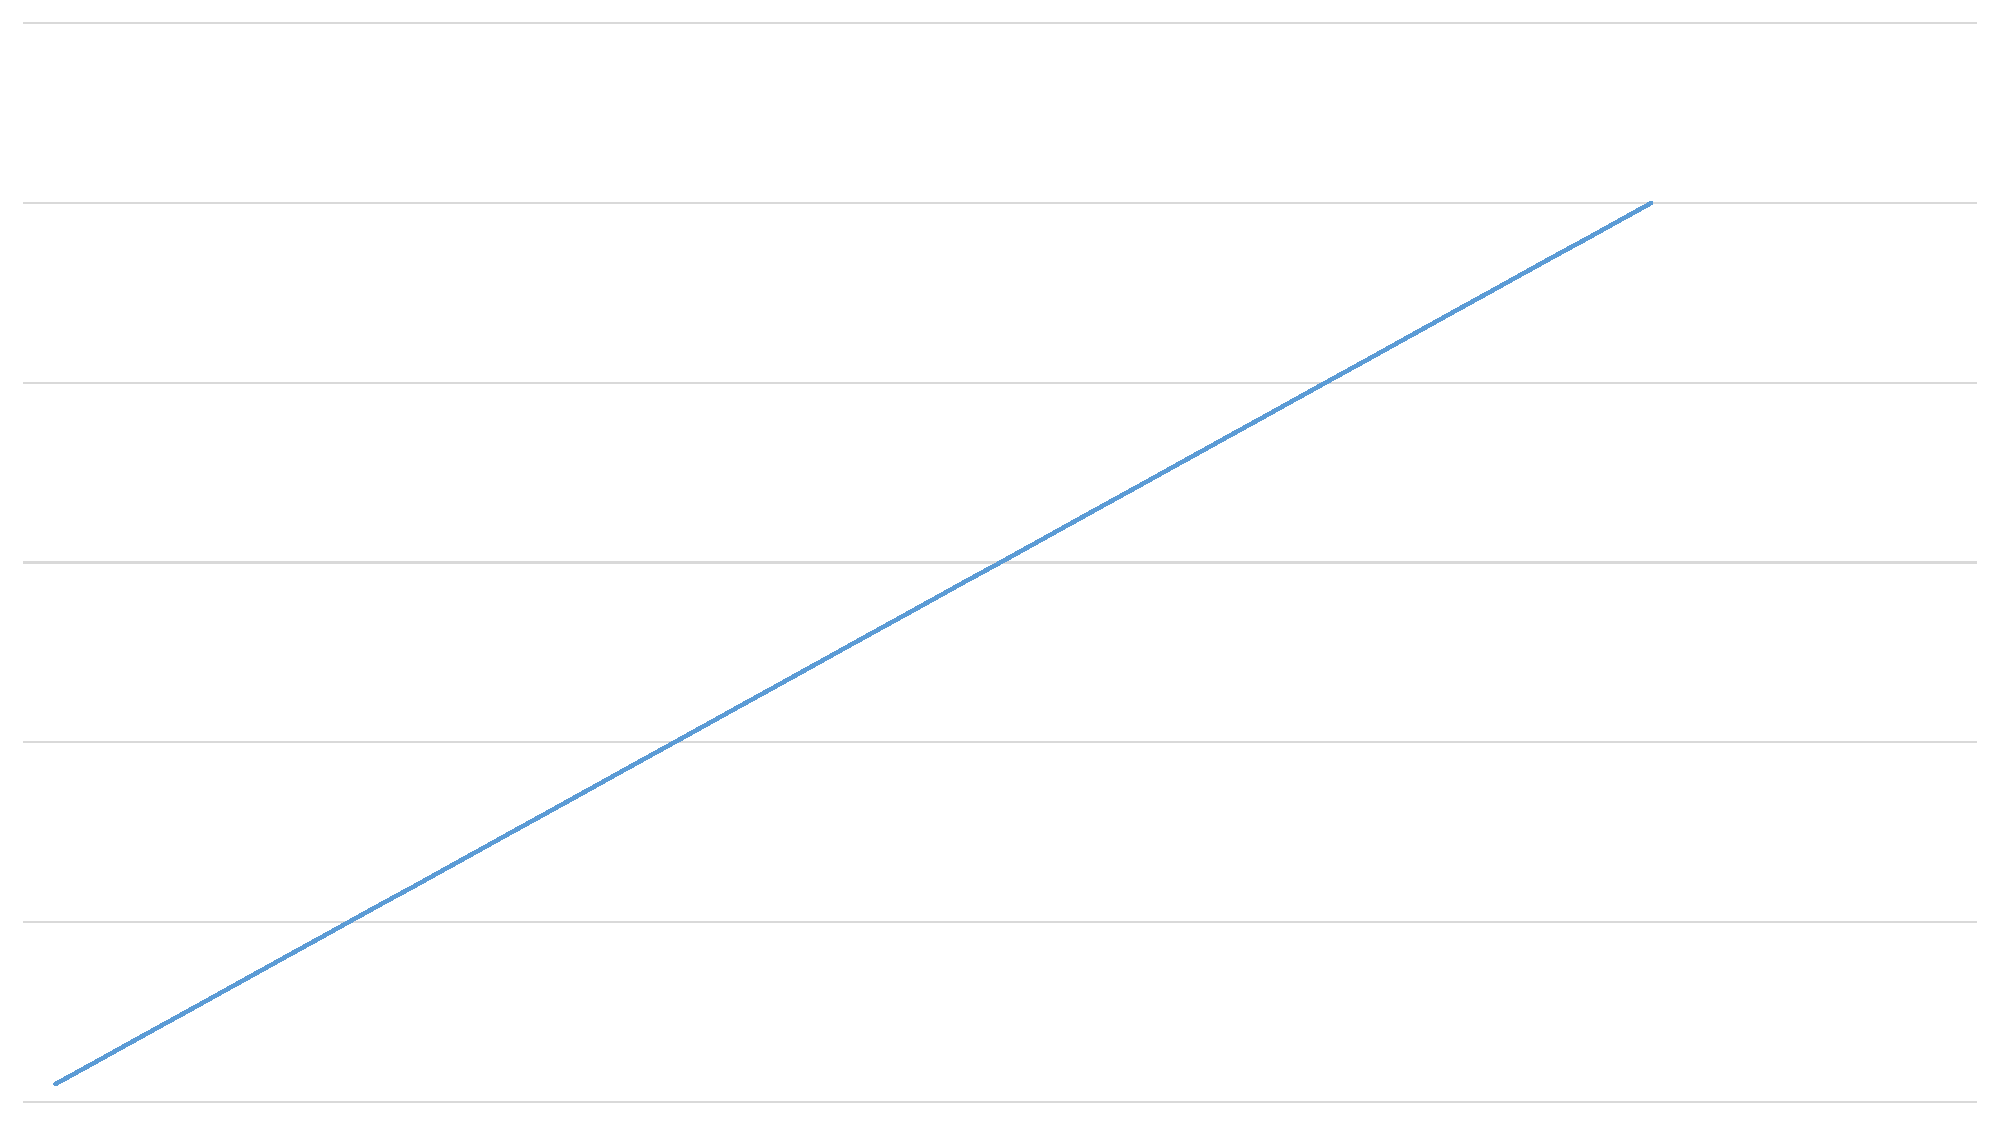
\includegraphics[width=13cm]{g1.pdf}
\caption{平均型}\label{g1}
\end{figure}

\subsection{急上昇型}
初期はあまり数値が伸びず停滞を続けるが,ある一点から数値が急速に伸び,上昇する.

\begin{figure}[htb]
\centering
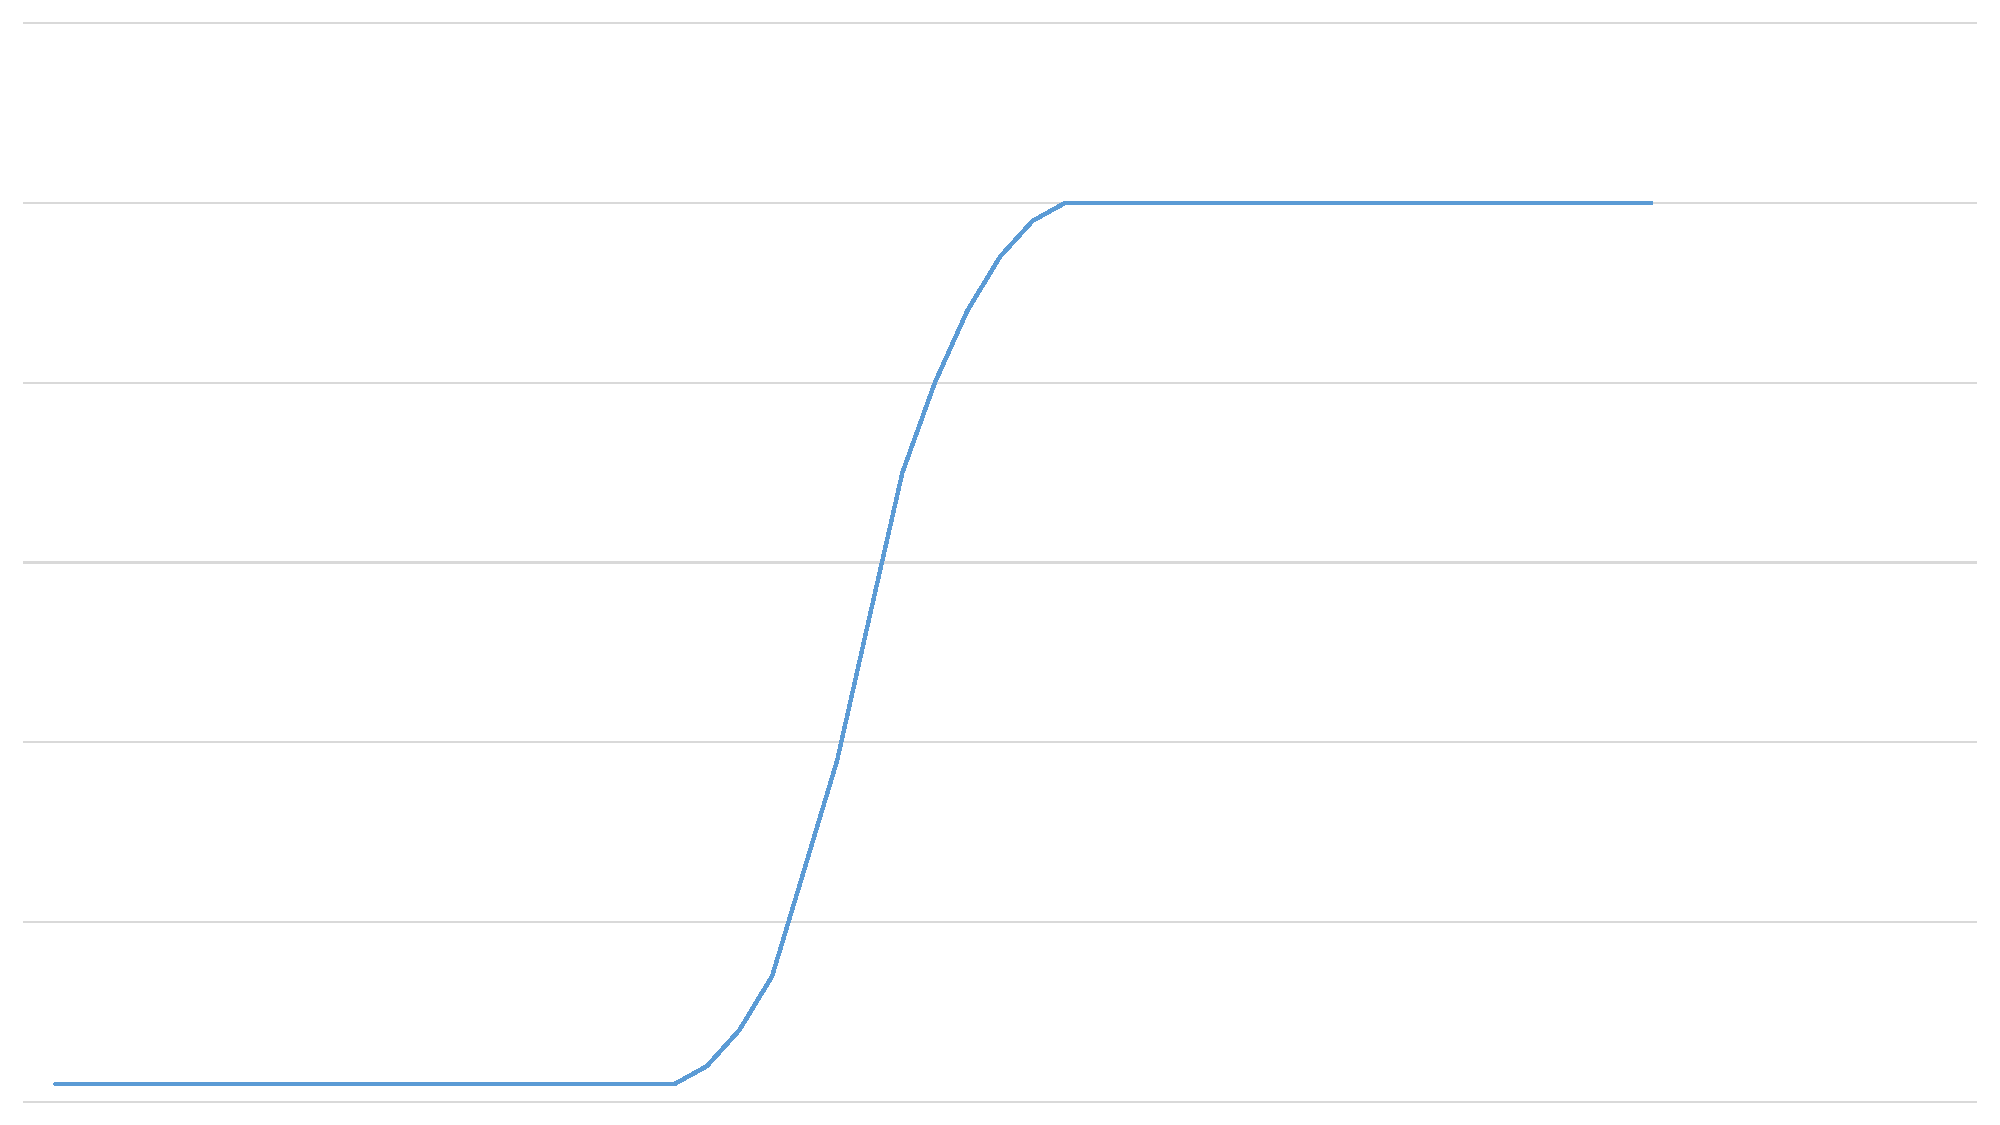
\includegraphics[width=13cm]{g2.pdf}
\caption{急上昇型}\label{g2}
\end{figure}

\newpage

\subsection{不規則型}

数値が上昇と停滞を繰り返し,波のような曲線を描く.

\begin{figure}[htb]
\centering
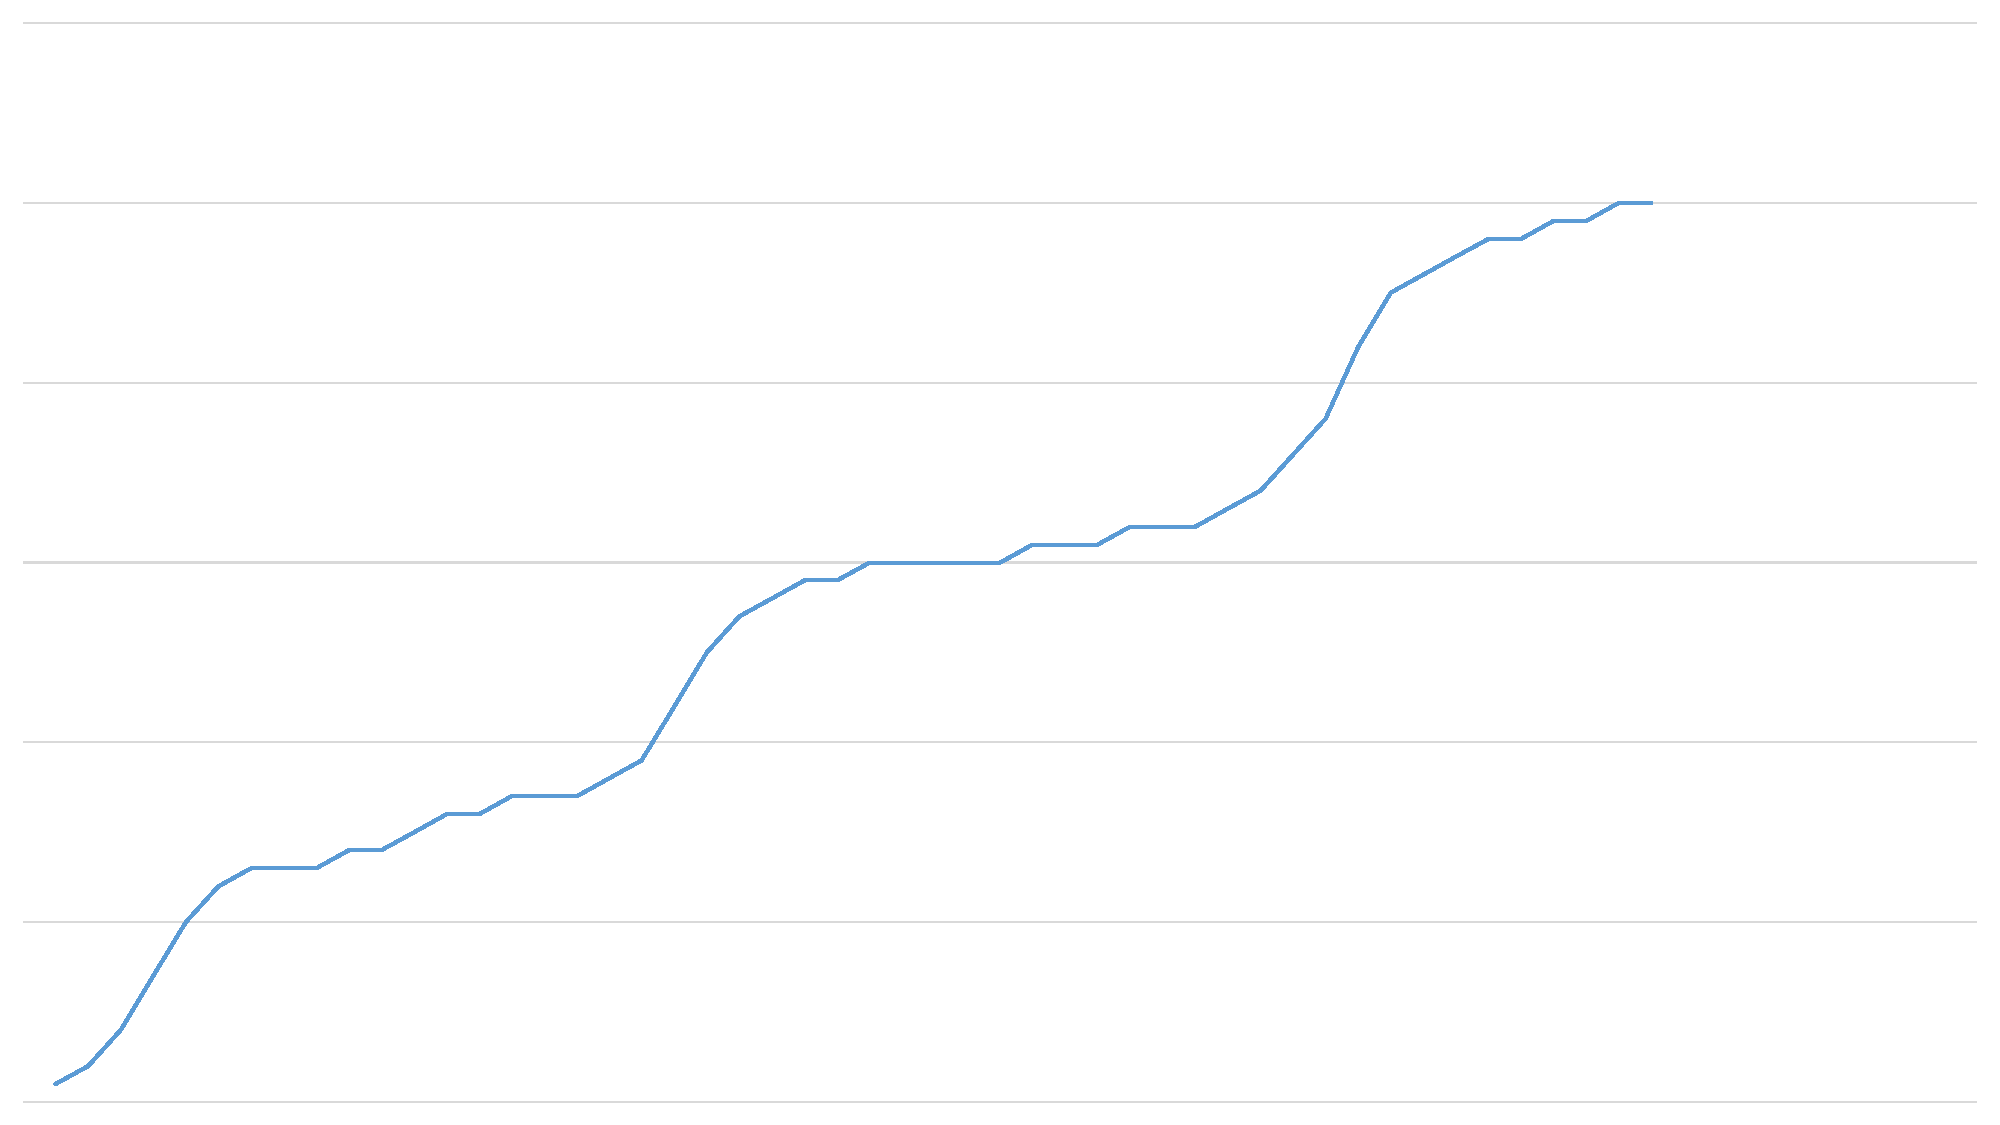
\includegraphics[width=13cm]{g3.pdf}
\caption{不規則型}\label{g3}
\end{figure}

\newpage

\section{各時刻ごとの増加数}
初めてエントリがブックマークがされてから24時間以内を対象に1時間ごとの時刻のブックマークの増加数を算出し,平均を求めた結果以下の表のような結果が得られた.


\begin{table}[htb]
\caption{時刻ごとの増加数の平均}\label{1t}
  \begin{tabular}{cr}
    時刻 & 増加数平均 \\
    1 & 5.76 \\
    2 & 4.53 \\
    3 & 2.41 \\
    4 & 1.89 \\
    5 & 2.97 \\
    6 & 4.66 \\
    7 & 9.74 \\
    8 & 15.5 \\
    9 & 17 \\
    10 &15.7  \\
    11 & 14.9  \\
    12 & 21.1 \\
    13 & 15.7 \\
    14 & 12.1 \\
    15 & 12.2 \\
    16 & 12 \\
    17 & 12.1 \\
    18 & 13.4 \\
    19 & 13.4 \\
    20 & 12.7 \\
    21 & 11.7 \\
    22 & 11.5 \\
    23 & 10.1 \\
    24 & 8.15 \\
  \end{tabular}
\end{table}

\newpage
\section{時間経過による増加数の変化}
初めてエントリがブックマークがされてから6時間ごとのブックマーク数増加数を算出した.
初めてのブックマークから24時間後のブックマーク数を100\%とし,各時間帯の増加率を求める.
その結果,以下の表のような結果となった.

\begin{table}[htb]
\caption{時刻の経過と増加率の平均}\label{1t}
  \begin{tabular}{cr}
    時刻の経過 & 増加率平均 \\
    6時間経過 & 22.39\% \\
    12時間経過 & 32.741\% \\
    18時間経過 & 27.854\% \\
    24時間経過 & 17.02\% \\
  \end{tabular}
\end{table}

以下のグラフは時刻の経過と増加率の平均を可視化したものである.

\begin{figure}[htb]
\centering
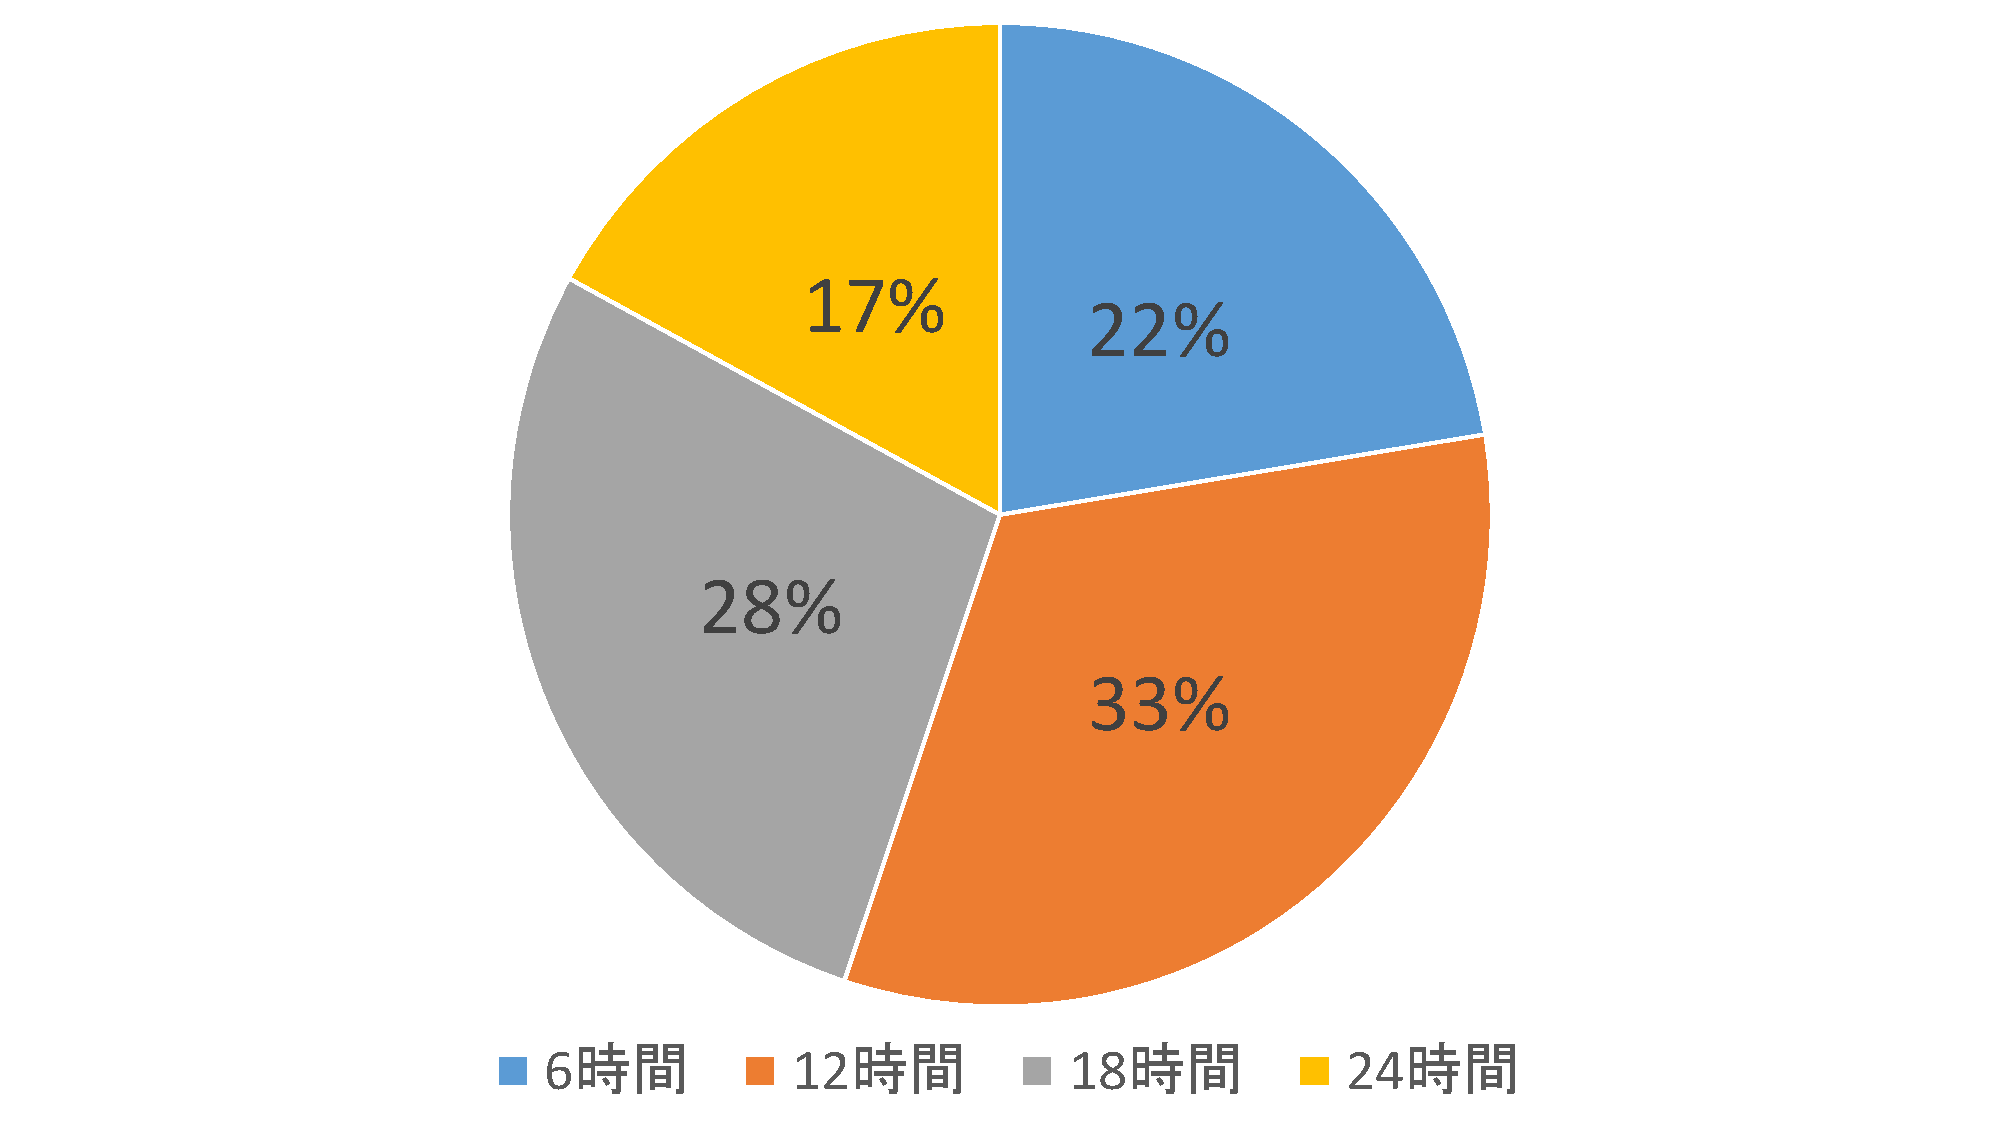
\includegraphics[width=10cm]{en.pdf}
\caption{時刻の経過と増加率の平均のグラフ}\label{en}
\end{figure}

\newpage

以下は時間の経過とブックマーク数と増加の例である.
\begin{figure}[htb]
\centering
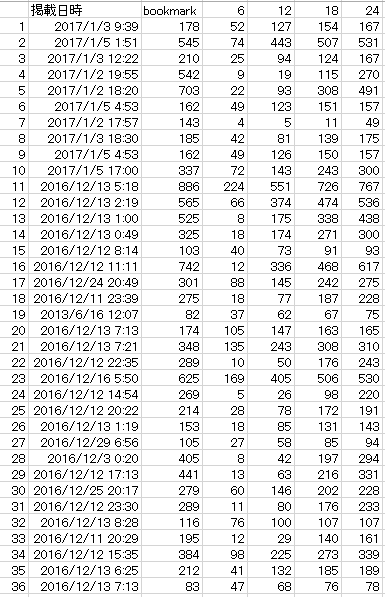
\includegraphics[width=10cm]{24.PNG}
\caption{時間の経過とブックマーク数}\label{24}
\end{figure}

\chapter{考察}
本章では分析結果をもとに考察を行っていく.

\section{ブックマークの伸びやすい時間帯についての考察}
分析結果からブックマーク数が伸びやすい時間帯は8時から13時まで伸びやすい時間帯であることが分かった.特に12時が最もブックマークの増加数が大きい時刻であった.朝起床してから新着のエントリを確認する人や昼の業務の合間の休憩時間にエントリを見る人が多いためだと推測される.\par
逆にブックマークの伸びにくい時間帯は2時から6時までであり,その中でも4時が最もブックマークの伸びにくい時刻であった.活動する人口が少ない深夜であることと,相対的にエントリをブックマークする人が少ないためエントリが共有されにくいことも要因と考えられる.

以下の画像は各時刻のブックマークの増加数の平均を可視化したものである.

\begin{figure}[htb]
\centering
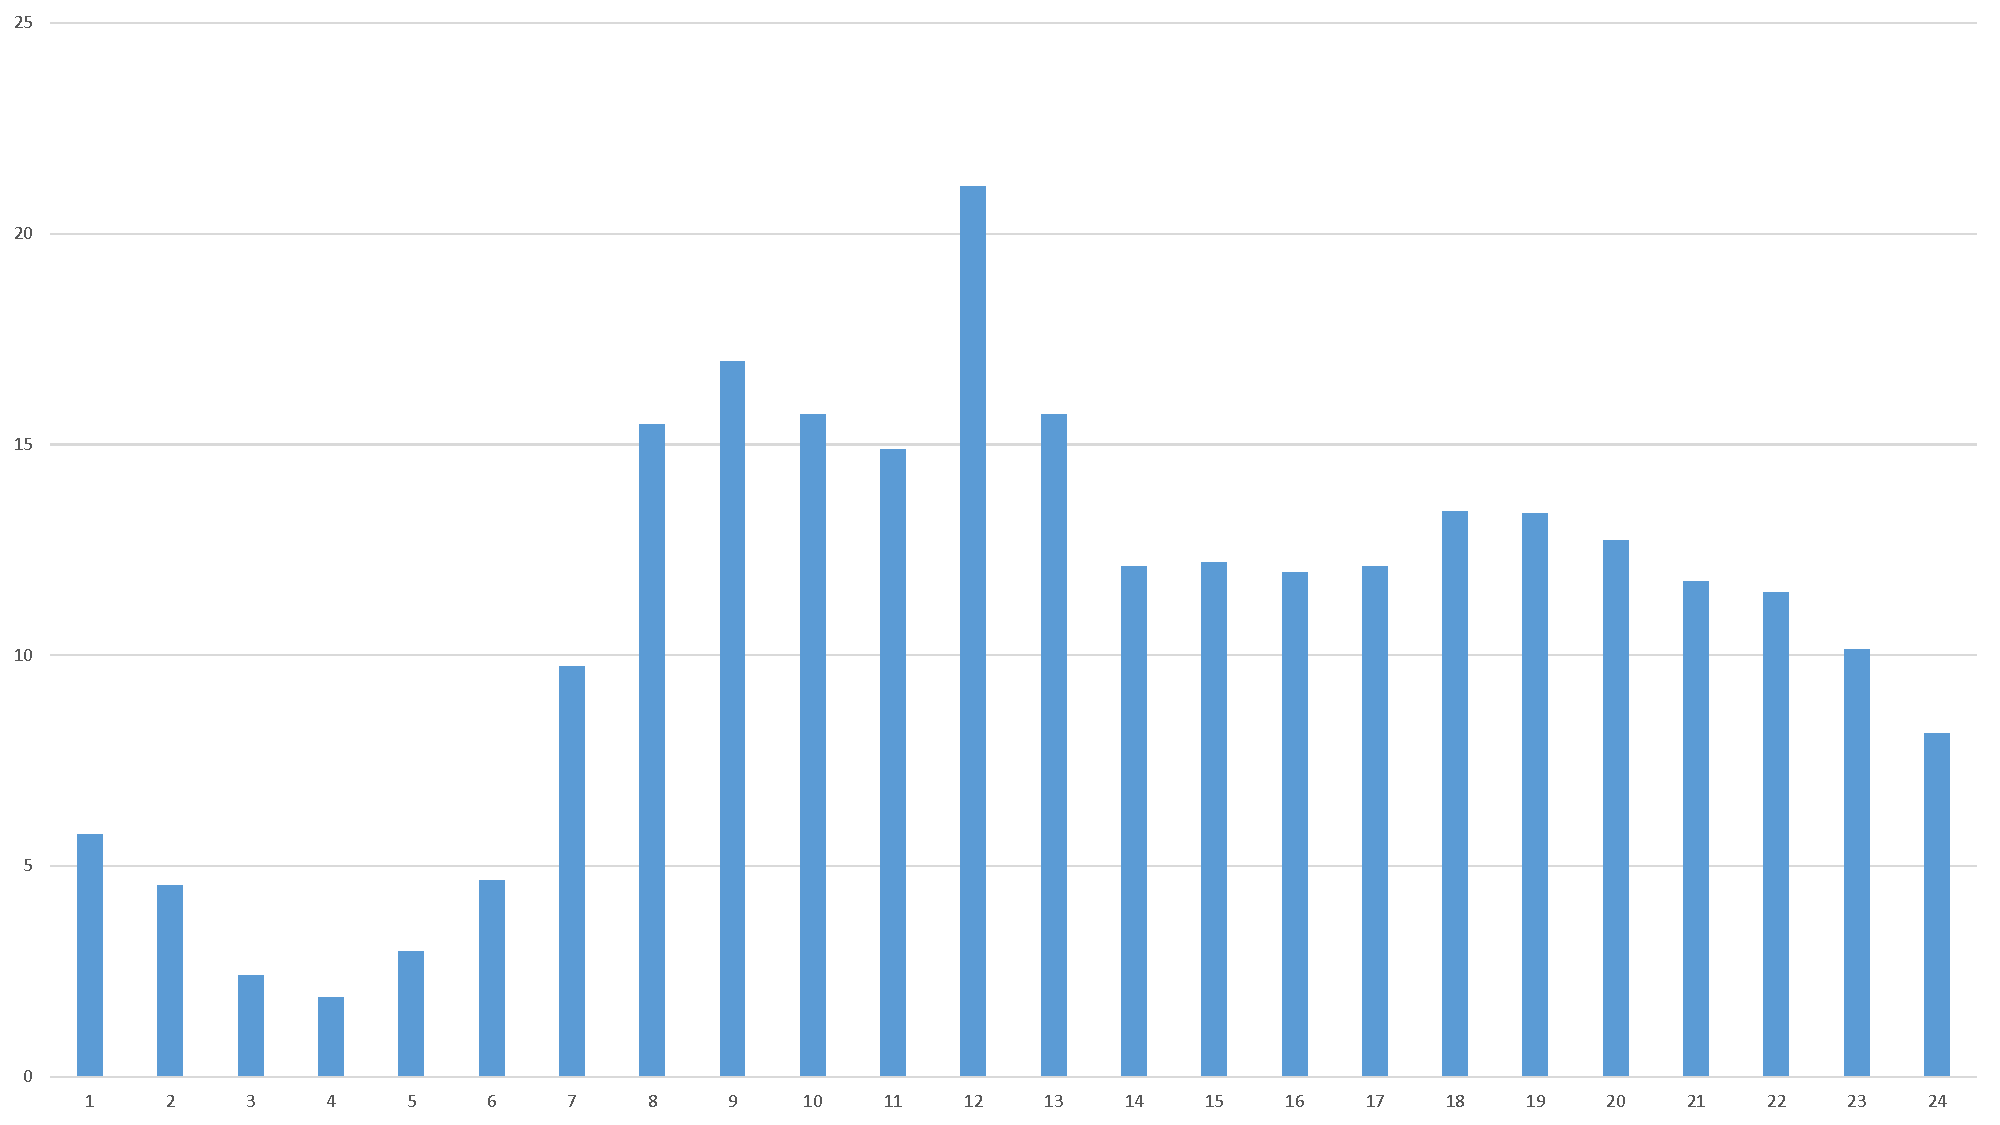
\includegraphics[width=13cm]{b-k.pdf}
\caption{各時刻のブックマークの増加数の平均}\label{bk}
\end{figure}

\newpage

\section{時間の推移に伴うブックマーク数の増加の傾向の考察}
3種類のグラフのパターンについて考察する.
\subsection{平均型}
この傾向は短期に急激にブックマーク数を伸ばしているものが多い.また日中にブックマークを伸ばし始めたものが多く,伸びにくい深夜に入る前の日中のうちにブックマーク数が伸びきってしまうためだと思われる.そのため停滞する区間がなく,変化の少ない曲線を描く.


\begin{figure}[htb]
\centering
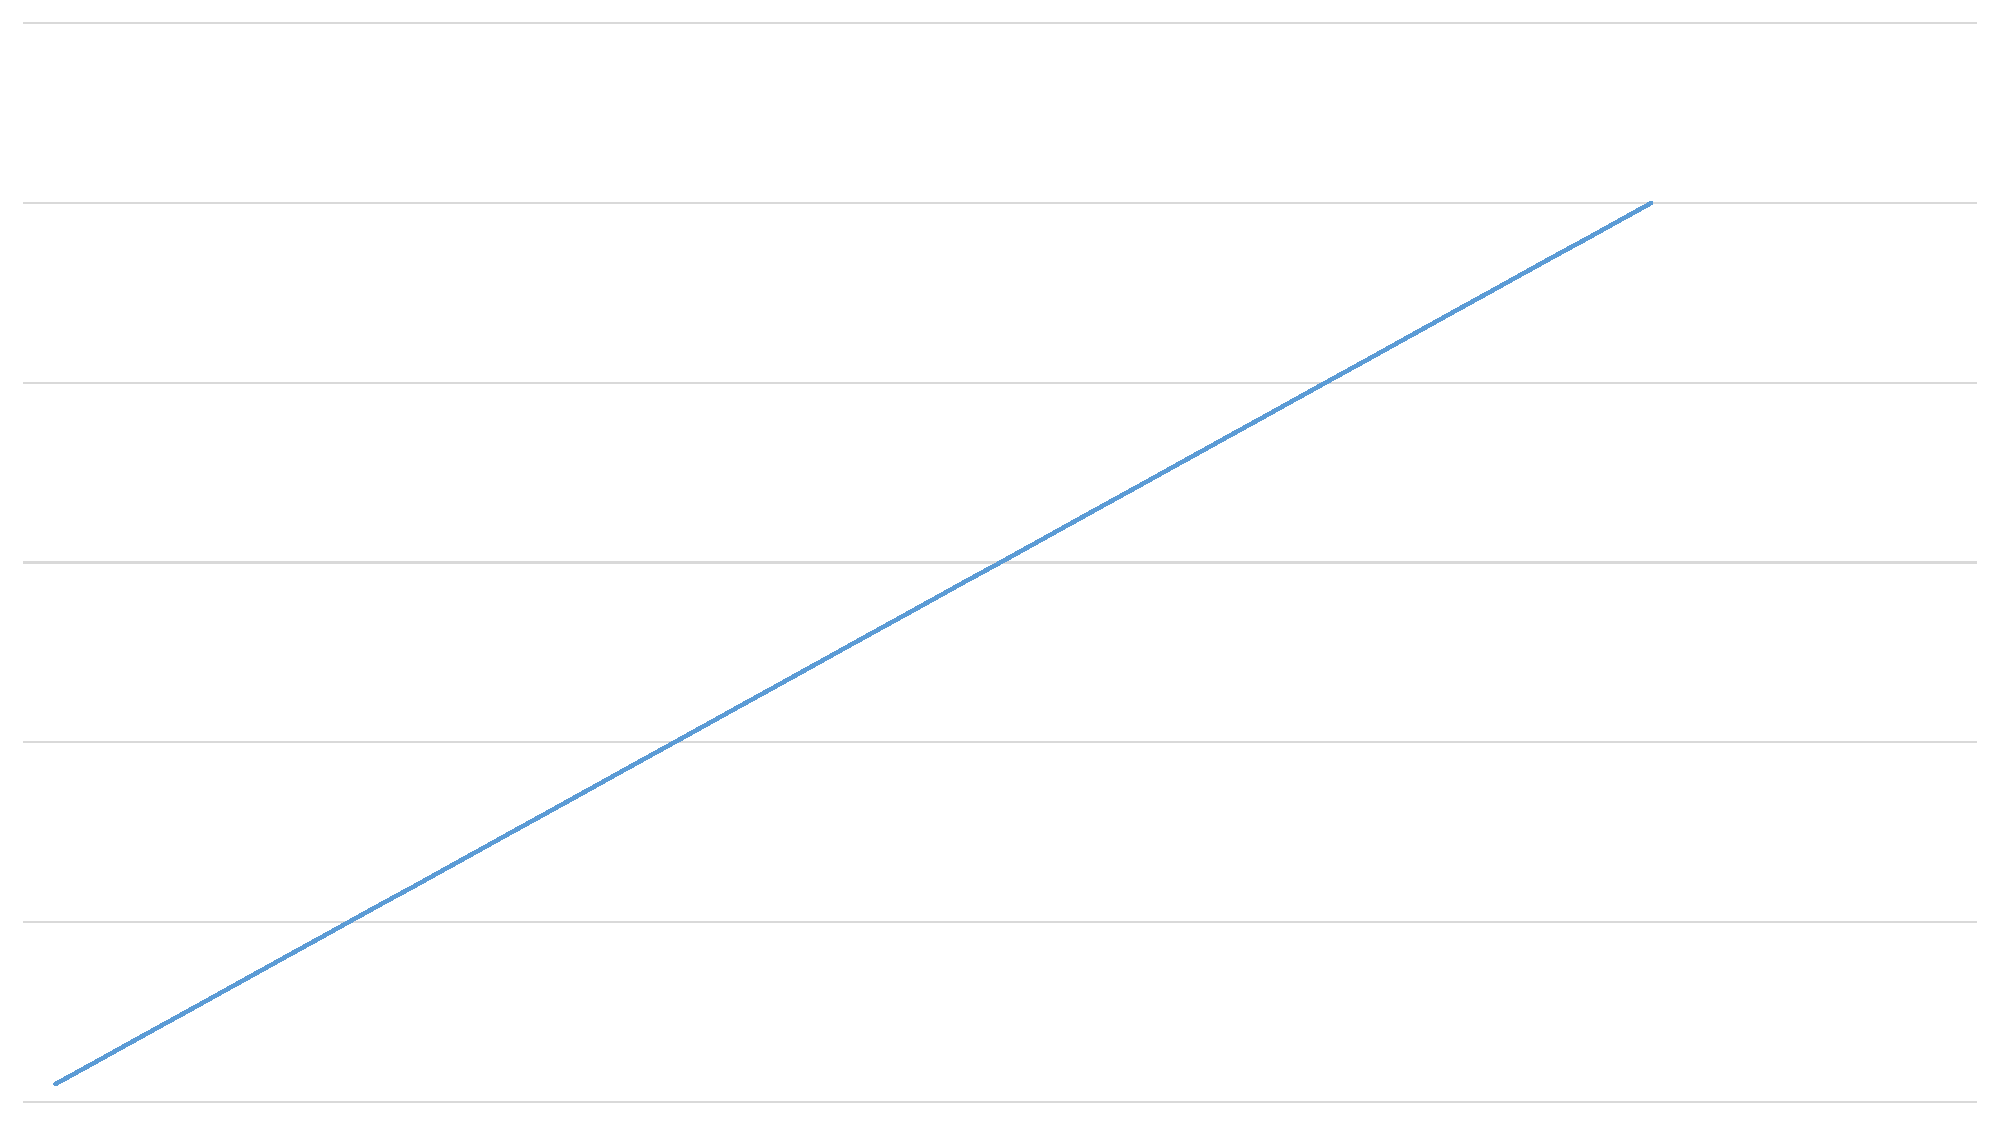
\includegraphics[width=13cm]{g1.pdf}
\caption{平均型}\label{g1}
\end{figure}

\newpage

\subsection{急上昇型}
この傾向は短期的にブックマーク数を伸ばしているもう一つの傾向であるが,平均型と異なり掲載日時が深夜のものが多い.深夜のためブックマーク数が伸びにくく初期の増加が停滞するが,人が活動を始める朝以降になるとブックマーク数を急速に伸ばし,結果急激に伸びる曲線を描いている.

\begin{figure}[htb]
\centering
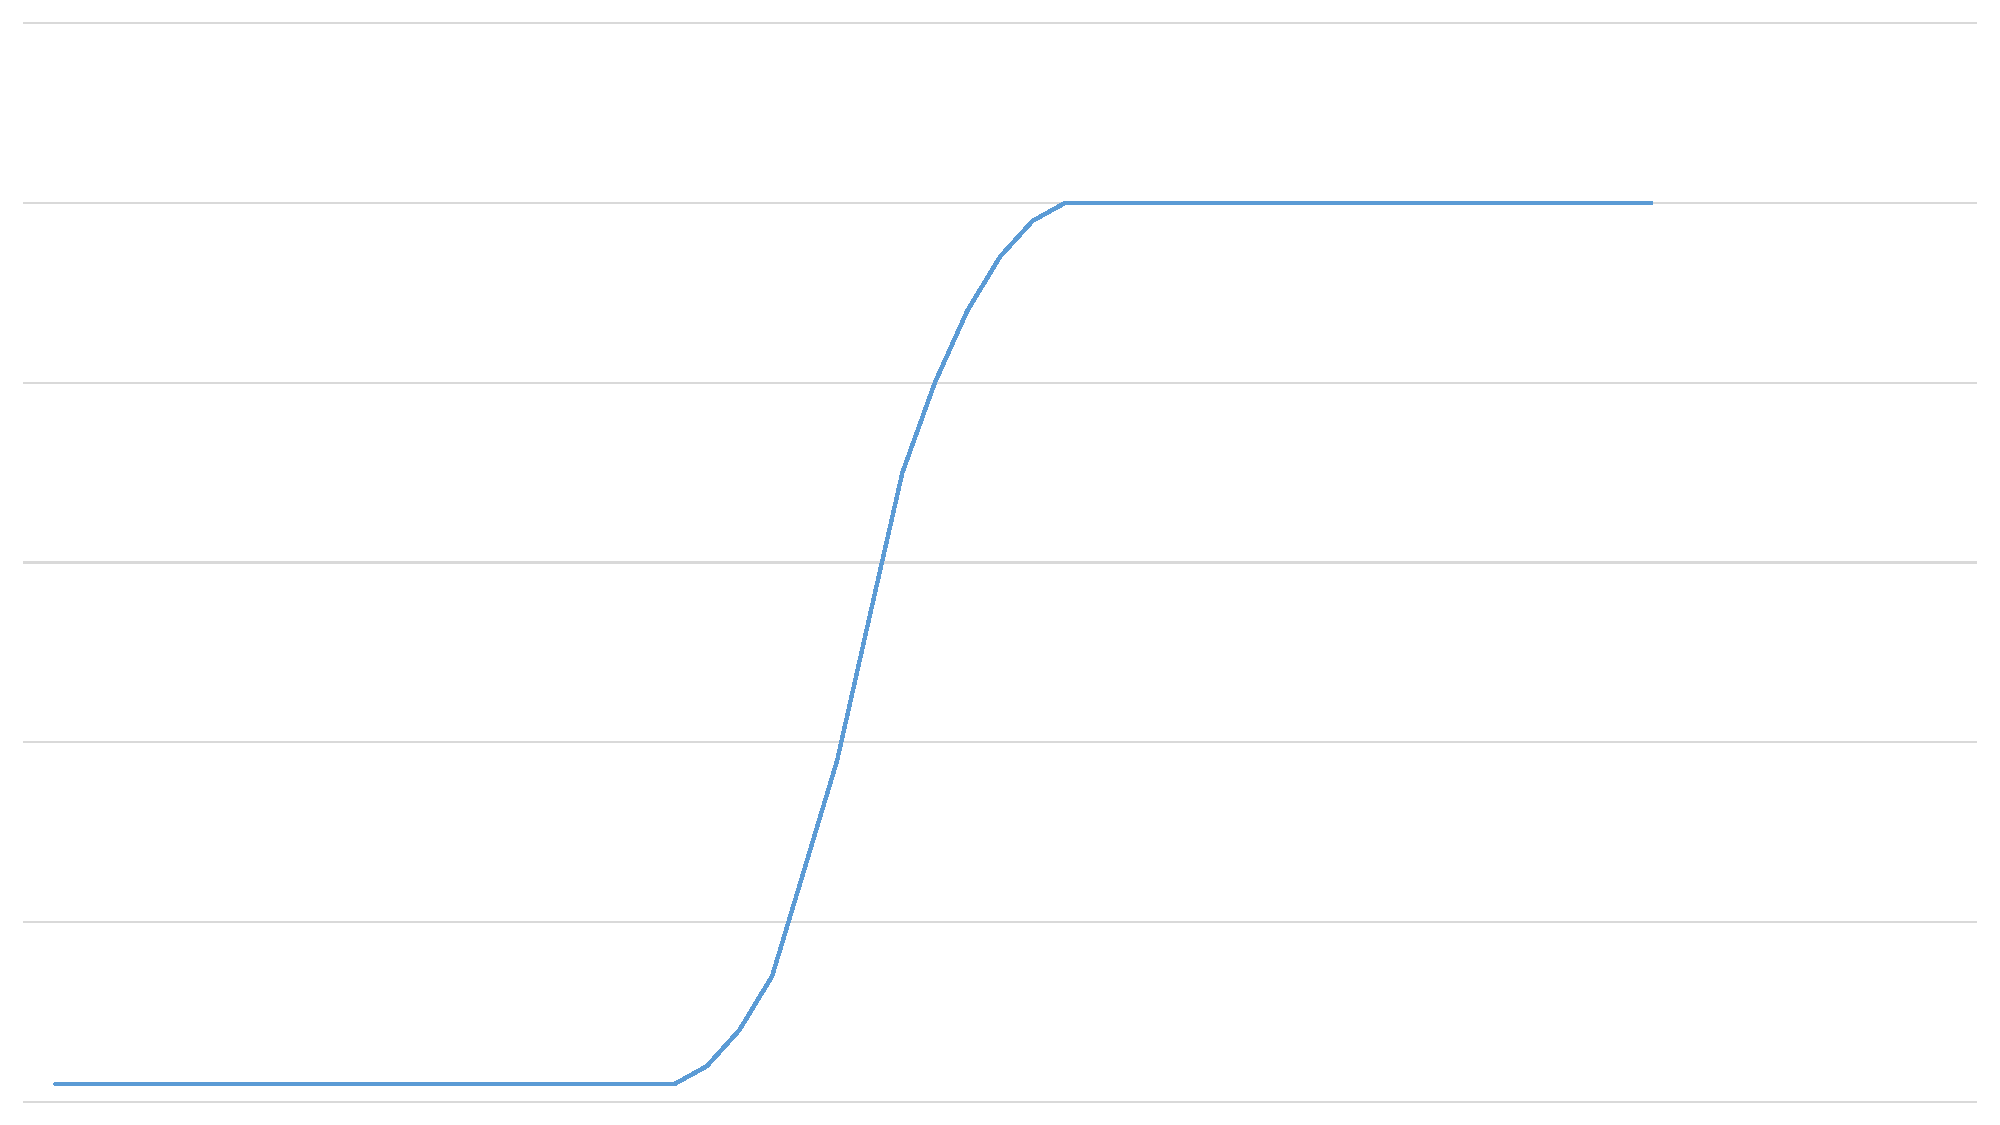
\includegraphics[width=13cm]{g2.pdf}
\caption{急上昇型}\label{g2}
\end{figure}

\newpage

\subsection{不規則型}
この傾向は長期的にブックマーク数を伸ばしているものに多い.長期にわたってブックマークを伸ばしているためその期間中にブックマーク数の伸びにくい深夜を数度挟んでいる.その結果停滞と上昇を繰り返し,波のような曲線を描いている.

\begin{figure}[htb]
\centering
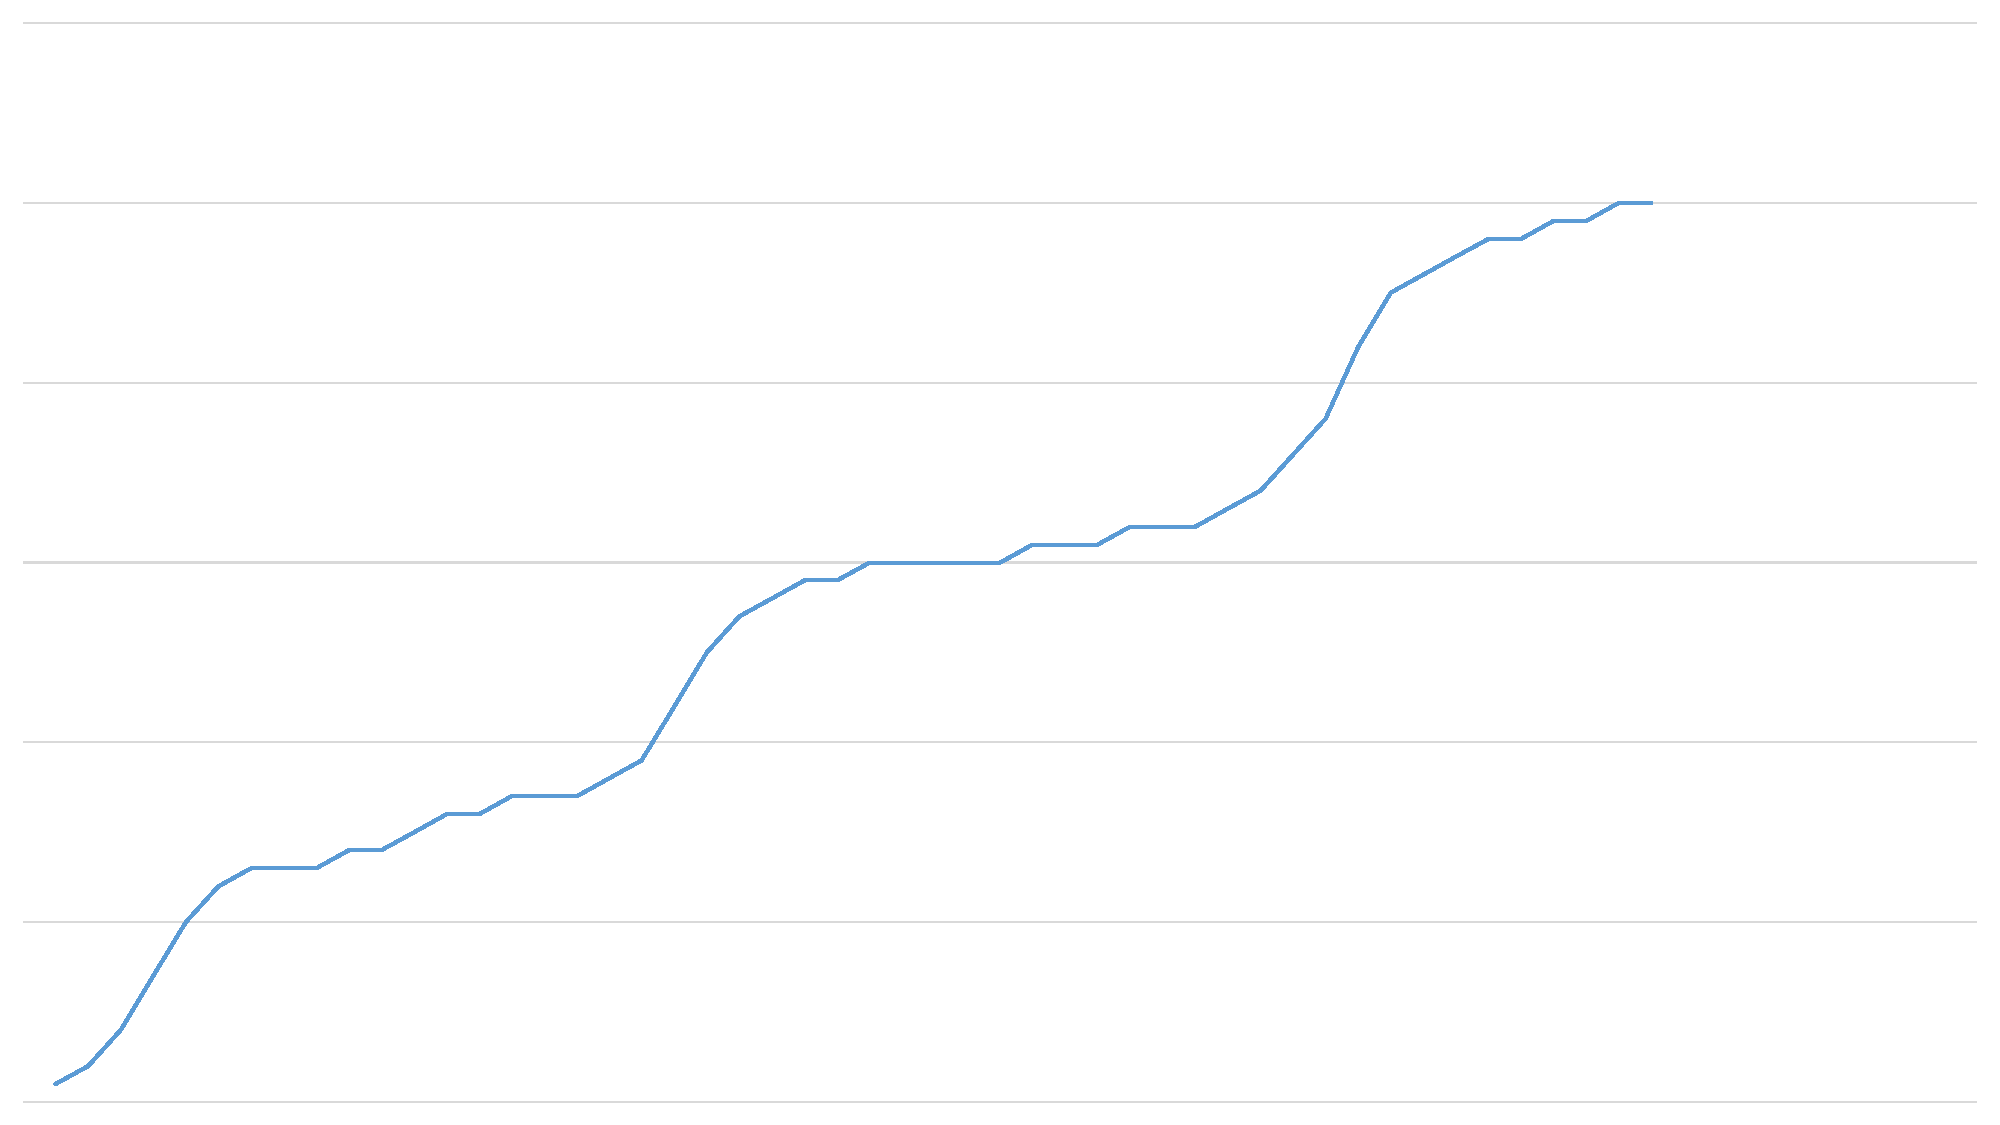
\includegraphics[width=13cm]{g3.pdf}
\caption{不規則型}\label{g3}
\end{figure}

\newpage

\section{時間経過による増加数の変化の考察}
分析の結果からそれぞれの時間帯に大きな差はないものの,傾向として6時間以上18時間未満に多く増加する傾向があることが分かった.特に6時間以上12時間未満での増加率が最も大きいことが分かった.\par
逆に18時間を超えると増加率は最も下がり,また差が小さいとはいえ初めの6時間も増加率が小さいことが分かった.\par
初めてのブックマークからあまり時間がたたない間はそこまで数が伸びにくく,ブックマークが本格的につき始めるためには数時間を要することが多いため,6時間以上12時間未満の時間帯の増加率が大きいのだと予測される.

\begin{figure}[htb]
\centering
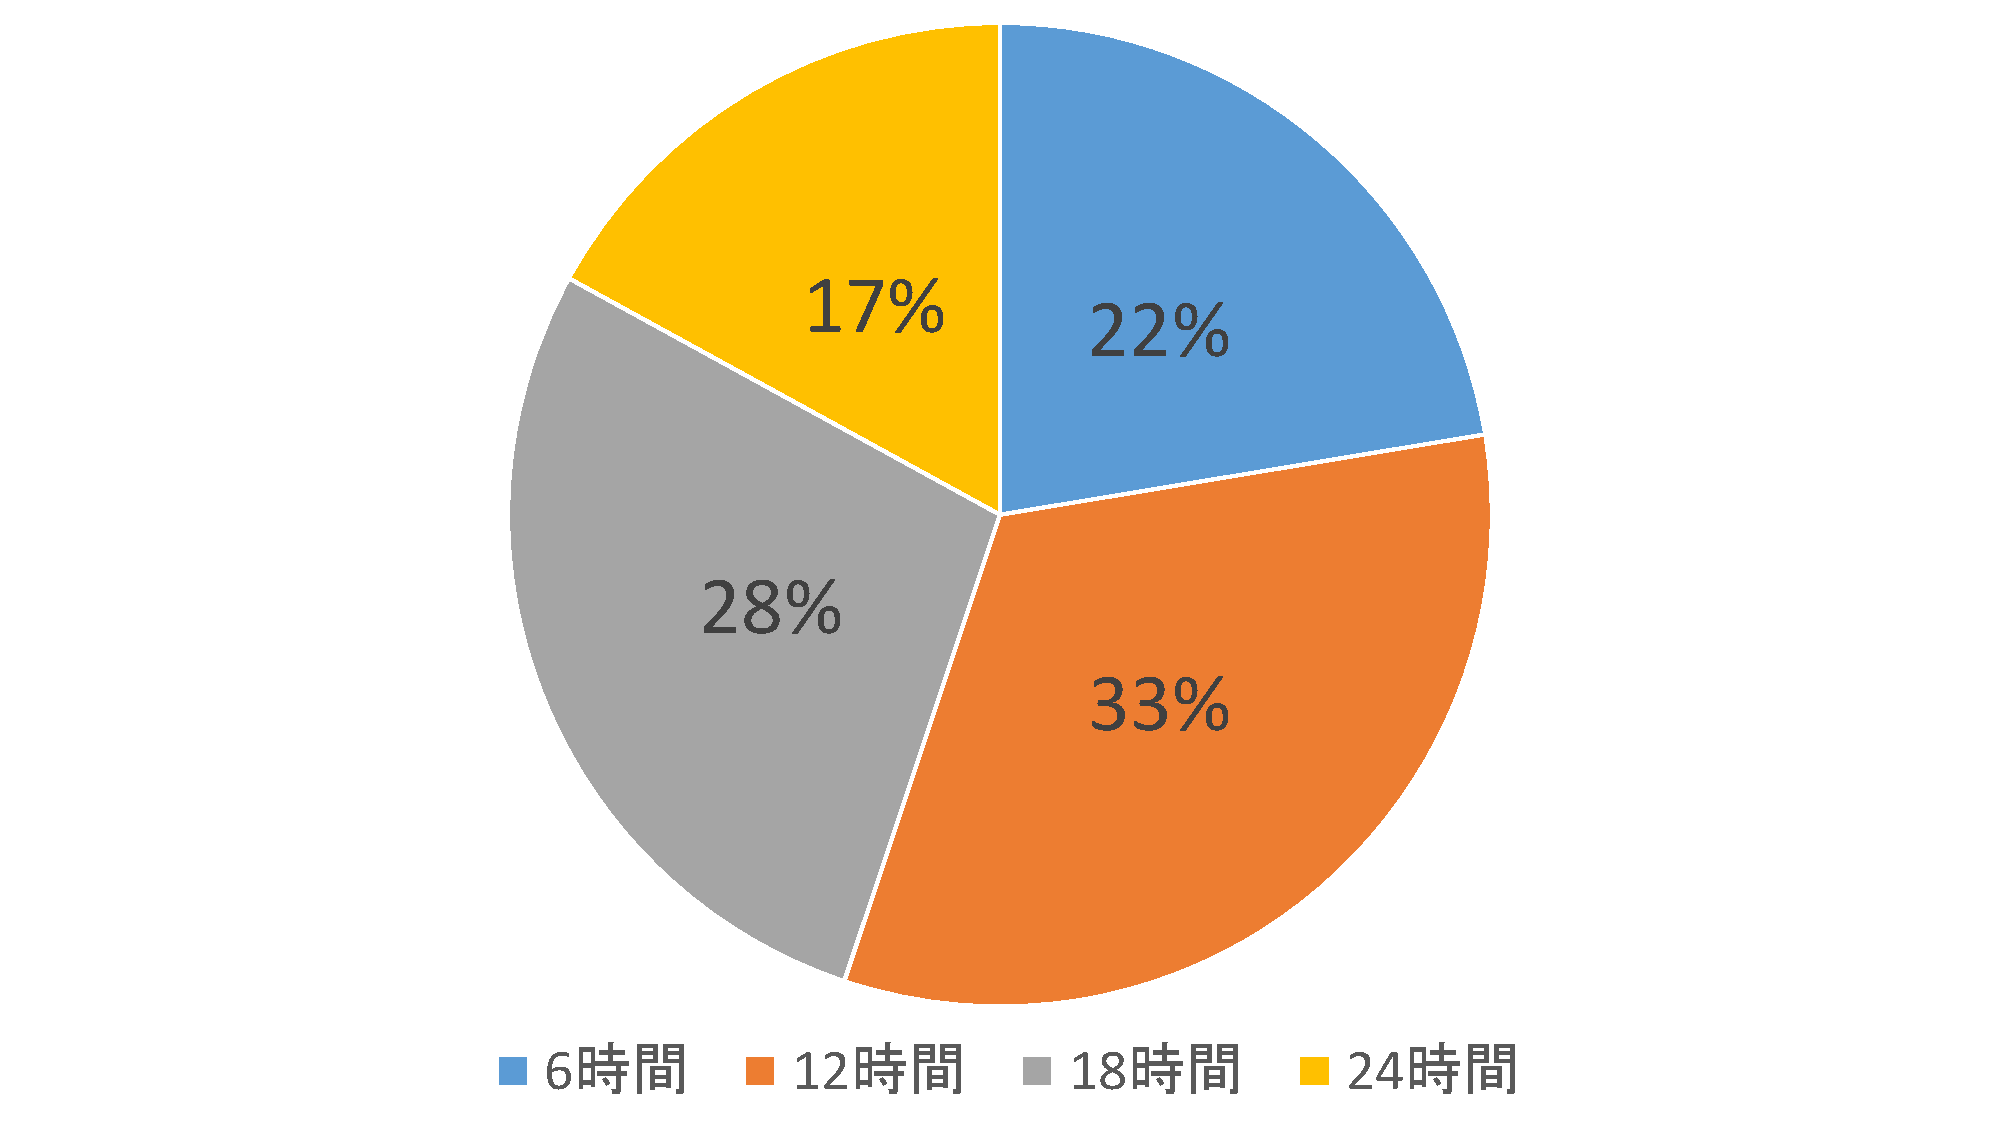
\includegraphics[width=15cm]{en.pdf}
\caption{時刻の経過と増加率の平均のグラフ}\label{en}
\end{figure}

\newpage

\section{3種の分析結果からの考察}
三種の分析結果から時間帯がブックマークの増加数に最も顕著に影響が出ていることが分かった.また時間の推移に伴うブックマーク数の増加の傾向についての可視化の結果と初回のブックマークからの時間経過による増加率から考察を行った.\par
その結果,朝の5時から7時程度までの間に初回のブックマークがつくようにすれば,昼には時間経過による増加率がピークを迎え,増加率の伸びにくい深夜に時間経過による増加率の少ない時間帯を重ねることができる.

\newpage

\chapter{結論}
本研究ではウェブマーケティングの例としてソーシャルブックマーケティングサービスを対象に,時間の推移に伴うブックマーク数の増加の傾向の分析を行い,ウェブマーケティングを行う上での指標の作成した.\par
分析の結果から時間帯によって大きくブックマーク数の増加の傾向が異なることが分かった.多く閲覧が見込める時間帯を意識しウェブマーケティングを行うことで,効果的なウェブマーケティングを行える確率が高まると思われる.\par
今回は時間とブックマーク数に着目し研究を行ったが,取得したが分析を行えなかった他の要素に関しても調査と分析を行い,それらの結果を組み合わせ多面的に考察を行うことでより精度の高いウェブマーケティングの予測と効果的なウェブマーケティングの手法の提案を行えることが期待できる.

\noindent
□□□□□□□□□■□□□□□□□□□■□□□□□□□□□■□□□□□□□□□■
□□□□□□□□□■□□□□□□□□□■□□□□□□□□□■□□□□□□□□□■
□□□□□□□□□■□□□□□□□□□■□□□□□□□□□■□□□□□□□□□■
□□□□□□□□□■□□□□□□□□□■□□□□□□□□□■□□□□□□□□□■
□□□□□□□□□■□□□□□□□□□■□□□□□□□□□■□□□□□□□□□■
□□□□□□□□□■□□□□□□□□□■□□□□□□□□□■□□□□□□□□□■
□□□□□□□□□■□□□□□□□□□■□□□□□□□□□■□□□□□□□□□■
□□□□□□□□□■□□□□□□□□□■□□□□□□□□□■□□□□□□□□□■
□□□□□□□□□■□□□□□□□□□■□□□□□□□□□■□□□□□□□□□■
□□□□□□□□□■□□□□□□□□□■□□□□□□□□□■□□□□□□□□□■
□□□□□□□□□■□□□□□□□□□■□□□□□□□□□■□□□□□□□□□■
□□□□□□□□□■□□□□□□□□□■□□□□□□□□□■□□□□□□□□□■
□□□□□□□□□■□□□□□□□□□■□□□□□□□□□■□□□□□□□□□■
□□□□□□□□□■□□□□□□□□□■□□□□□□□□□■□□□□□□□□□■
□□□□□□□□□■□□□□□□□□□■□□□□□□□□□■□□□□□□□□□■
□□□□□□□□□■□□□□□□□□□■□□□□□□□□□■□□□□□□□□□■
□□□□□□□□□■□□□□□□□□□■□□□□□□□□□■□□□□□□□□□■
□□□□□□□□□■□□□□□□□□□■□□□□□□□□□■□□□□□□□□□■
□□□□□□□□□■□□□□□□□□□■□□□□□□□□□■□□□□□□□□□■
□□□□□□□□□■□□□□□□□□□■□□□□□□□□□■□□□□□□□□□■
□□□□□□□□□■□□□□□□□□□■□□□□□□□□□■□□□□□□□□□■
□□□□□□□□□■□□□□□□□□□■□□□□□□□□□■□□□□□□□□□■
□□□□□□□□□■□□□□□□□□□■□□□□□□□□□■□□□□□□□□□■
□□□□□□□□□■□□□□□□□□□■□□□□□□□□□■□□□□□□□□□■
□□□□□□□□□■□□□□□□□□□■□□□□□□□□□■□□□□□□□□□■
□□□□□□□□□■□□□□□□□□□■□□□□□□□□□■□□□□□□□□□■
□□□□□□□□□■□□□□□□□□□■□□□□□□□□□■□□□□□□□□□■
□□□□□□□□□■□□□□□□□□□■□□□□□□□□□■□□□□□□□□□■
□□□□□□□□□■□□□□□□□□□■□□□□□□□□□■□□□□□□□□□■
□□□□□□□□□■□□□□□□□□□■□□□□□□□□□■□□□□□□□□□■
□□□□□□□□□■□□□□□□□□□■□□□□□□□□□■□□□□□□□□□■
□□□□□□□□□■□□□□□□□□□■□□□□□□□□□■□□□□□□□□□■
□□□□□□□□□■□□□□□□□□□■□□□□□□□□□■□□□□□□□□□■
□□□□□□□□□■□□□□□□□□□■□□□□□□□□□■□□□□□□□□□■
□□□□□□□□□■□□□□□□□□□■□□□□□□□□□■□□□□□□□□□■
□□□□□□□□□■□□□□□□□□□■□□□□□□□□□■□□□□□□□□□■
□□□□□□□□□■□□□□□□□□□■□□□□□□□□□■□□□□□□□□□■
□□□□□□□□□■□□□□□□□□□■□□□□□□□□□■□□□□□□□□□■
□□□□□□□□□■□□□□□□□□□■□□□□□□□□□■□□□□□□□□□■
■■■■■■■■■■■■■■■■■■■■■■■■■■■■■■■■■■■■■■■■
□□□□□□□□□■□□□□□□□□□■□□□□□□□□□■□□□□□□□□□■

\bibliographystyle{junsrt}
\bibliography{biblio}%「biblio.bib」というファイルが必要.


\end{document}
